\chapter{Calcul des coefficients pour un plan infini}
\label{sec:plan}
\minitoc
\newpage

\sectionstar{Introduction}
Pour déterminer des coefficients complexes satisfaisants aux conditions introduites dans la partie précédente, nous commençons par la méthode de l'approximation du plan tangent, documenté par \cite{hoppe_impedance_1995,marceaux_high-order_2000,aubakirov_electromagnetic_2014}.
Cette méthode consiste à considérer localement l'objet, supposé régulier, comme son plan tangent comme un plan infini, ce qui reste valable dans le cadre de cette thèse, car nos objets d'études sont parfaitement réguliers.

Nous rappellerons l'opérateur de Calderón exact qui lie les champs électromagnétiques à la surface extérieure de l’objet, ainsi que la condition nécessaire pour l'obtenir.
Pour des considérations de mise en œuvre numérique, nous présenterons une méthode itérative pour exprimer cet opérateur.
Cette dernière va ajouter des conditions, dont nous rappellerons qu'elles ne sont à considérer que dans le cadre de cette méthode itérative.

\section{Analyse de Fourier de l'opérateur d'impédance}

Des résultat sur l'analyse spectrale de l'opérateur d'impédance ont déjà été présenté par \cite{hoppe_impedance_1995} pour des conducteurs plans et cylindriques recouvert d'une couche de matériau.
Nous les rappellerons ainsi la méthode pour les obtenir puis nous montrerons que étendre ces résultats à plusieurs couches est immédiat. 
% De plus, nous feront intervenir les matrices associées aux opérateurs \(\LD,\LR\) dans ces résultats.

% \TODO{
%     Généraliser ce qui suit à des matériaux non borné à l'aide de fonctions rapidement décroissantes
% }

Soit \(\OO\) un domaine fermé, bornée, de frontière régulière. Supposons que ces champs soient \(L^2\) en espace et en temps: \((\vE(\vect{x},t),\vH(\vect{x},t)) \in L^2(\OO \times \RR_+) \cap L^2(\OO^c\times\RR_+)\) et vérifient les équations de Maxwell:
\begin{equation}
    \left\lbrace
    \begin{matrix}
    \vrot \vE(\vect{x},t) &=& -\mu(\vx) \ddr{t}{\vH}(\vx,t) \\
    \vrot \vH(\vect{x},t) &=& \eps(\vx) \ddr{t}{\vE}(\vx,t)
    \end{matrix}
    \right.
\end{equation}

On suppose aussi que \(\eps\) et \(\mu\) sont constant par morceaux.

Puisque ces champs \(\vE(\vect{x},t),\vH(\vect{x},t)\) sont \(L^2\), on peut définir leurs transformées de Fourier \(\hat{\vE}(\vect{k},\w), \hat{\vH}(\vect{k},\w)\) (\cite[Théorème de Plancherel, p.~153]{yosida_functional_1995}) telle que

\begin{equation}
    \hat{\vE} (\vect{k},\w) = \frac{1}{\sqrt{2\pi}^3}\int_{\RR^3\times\RR_+} e^{-i(\vect{k} \cdot \vect{x}+\w t)}\vE(\vect{x},t) \dd{x}\dd{t}\,, \quad \dd x = \prod\limits_{i=1}^3 \dd{x}_i
\end{equation}
\begin{equation}
    \vE(\vect{x},t) = \frac{1}{\sqrt{2\pi}^3}\int_{\RR^3\times\RR_+} e^{i(\vect{k} \cdot \vect{x}+\w t)}\hat{\vE} (\vect{k},\w) \dd{k} \dd{\w}\,, \quad \dd k = \prod\limits_{i=1}^3 \dd{k}_i
\end{equation}
La méthode pour trouver une expression de l'opérateur d'impédance est la suivante.
\begin{itemize}
\item Faire une transformée de Fourier partielle des champs, dépendante de la géométrie.
\item Réécrire le système d'équation de Maxwell simplifié.
\item Obtenir des EDO simple à résoudre sur les composantes des champs.
\item Utiliser les conditions limites pour obtenir les solutions particulières de cette EDO.
\item En déduire l'opérateur d'impédance en Fourier.
\end{itemize}

Dans ce qui suit, on réalise au moins une transformée partielle en temps. La variable de Fourier associée est \(\w\), et donc l'opérateur \(\ddr{t}{~}\) est remplacé par \(i\w\).

% \begin{tcolorbox}
% On ne différencie pas les champs \(\vE,\vH\) de leurs transformées de Fourier \(\hat \vE, \hat \vH\).
% \end{tcolorbox}

On va donc utiliser le système d'équations de Maxwell harmonique:
\begin{equation}
    \left\lbrace
    \begin{matrix}
    \vrot \hat \vE(\vx,\w)  &=& -i \omega \mu \hat \vH(\vx,\w)  \\
    \vrot \hat \vH(\vx,\w)  &=& i \omega \eps \hat \vE(\vx,\w)
    \end{matrix}
    \right.
    \label{eq:imp_fourier:intro:maxwell_harmonique}
\end{equation}

A partir de maintenant, la dépendance en \(\w\) sera implicite: \(\hat \vE(\vx) \equiv \hat \vE (\vx, \w)\).
\section{Expressions exactes des matrices d'impédance et des matrices de réflexions pour un plan infini}
    % Ce cas est très bien documenté (\cite{senior_approximate_x995},\cite{hoppe_impedance_x995}) et pose la méthodologie à adopter pour les objets courbes.

    Dans un premier temps, on peut sans perte de généralités faire une rotation du repère pour avoir le plan orthogonal à \(\vect{z}\).

    \begin{figure}[!h]
        \begin{center}
            \tikzsetnextfilename{plan_1_couche}
            \begin{tikzpicture}
                \input{tikz/schema/plan_1_couche.tikz}
            \end{tikzpicture}
        \end{center}
    \end{figure}

    % Comme il est infini dans les directions \(\vect{e_x} ,\vect{e_y}\) et que le matériau est homogène isotrope, 
    Nous utilisons une transformée partielle en \(x, y\).

    \begin{equation}
        \vE(x,y,z) = \frac{1}{2\pi}\iint_{\RR^2} e^{i(k_x x + k_y y)}\hat{\vE} (k_x,k_y,z) \dd{k_x}\dd{k_y}
    \end{equation}

    Grâce à cela, nous simplifions le problème en étudiant \( \hat{\vE}\) grâce aux multiplicateurs de Fourier associés aux variables \(x,y\). 

    \begin{defn}
        Soient \((k_x,k_y) \in \RR^2\) fixé.
        Soit \(k_3\) la fonction constante par morceaux en \(z\) telle que
        \begin{equation*}
          \fonction{k_3}{[-d,\infty[}{\CC}
          {z}{\sqrt{\w^2\eps(z)\mu(z) - k_x^2 - k_y^2}}
        \end{equation*}
        Par abus de notation, on omettra les dépendances en \(z\) pour \(k_3\).
    \end{defn}

    \begin{prop}
        On se place dans le matériau et on suppose que \(\forall z \in [-d,0], k_3(z) \not = 0\).
        Alors existe \((c_i(k_x,k_y))_{1\le i \le4}, \in \CC(\RR^2)^4\) tels que
        \begin{subequations}
            \begin{align}
                \hat{E}_y(k_x,k_y,z) & = e^{ik_3(z)z}c_1(k_x,k_y) + e^{-ik_3(z)z}c_2(k_x,k_y)
                \\
                \hat{H}_y(k_x,k_y,z) & = e^{ik_3(z)z}c_3(k_x,k_y) + e^{-ik_3(z)z}c_4(k_x,k_y)
            \end{align}
        \end{subequations}
    \end{prop}

    \begin{proof}
      On commence par coupler les équations de Maxwell pour obtenir des équations sur chaque champ seul
      \begin{align*}
          \vlapl{\vE} + \w^2\eps(z)\mu(z) \vE & = 0
          \\
          \vlapl{\vH} + \w^2\eps(z)\mu(z) \vH & = 0
      \end{align*}
      On pose \(k(z)^2=\w^2\eps(z)\mu(z)\)

      Donc chaque composante de chaque champ est solution d'une équation de Helmholtz. On s’intéresse alors à la composante en \(y\) seulement:
      \begin{align*}
          \lapl{E_y} + k(z)^2 E_y & = 0
          \\
          \lapl{H_y} + k(z)^2 H_y & = 0
      \end{align*}

      Si l'on applique ces équations différentielles aux transformées de Fourier, on obtient
      \begin{align*}
          \ddr[2]{z}{\hat{E}_y}(k_x,k_y,z) + \left( k(z)^2 - k_x^2 - k_y^2\right) \hat{E}_y(k_x,k_y,z) & = 0
          \\
          \ddr[2]{z}{\hat{H}_y}(k_x,k_y,z) + \left( k(z)^2 - k_x^2 - k_y^2\right) \hat{H}_y(k_x,k_y,z) & = 0
      \end{align*}

      On suppose alors que \(k_3^2\) ne s'annule pas dans la couche. S'il s'annule, les solutions sont linéaire en \(z\) et nous référons à l'annexe \ref{sec:annexe:plan:k3_nul}.

      Une solution générale s'écrit alors
      \begin{align*}
          \hat{E}_y(k_x,k_y,z) & = e^{ik_3(z)z}c_1(k_x,k_y) + e^{-ik_3(z)z}c_2(k_x,k_y)
          \\
          \hat{H}_y(k_x,k_y,z) & = e^{ik_3(z)z}c_3(k_x,k_y) + e^{-ik_3(z)z}c_4(k_x,k_y)
      \end{align*}
    \end{proof}

    % Ce choix est motivé par l'invariance par rotation du plan infini. Or il est d'usage de la représenter comme sur le schéma, avec un propagation de l'onde dans le plan \(xOz\). Souvent, on parle alors de polarisation pour simplifier les calculs. En effet, une polarisation \gls{acr-te} consiste à dire que \(\vE\) n'a qu'une composante dans le plan transverse au plan de propagation, donc suivant \(\vect{e_y}\). De même une polarisation \gls{acr-tm} consiste à dire que \(\vH\) n'a qu'une composante suivant \(\vect{e_y}\). C'est ce qui motive ce choix absolument abstrait d'utiliser les deuxièmes composantes.

    \subsection{Expressions des champs tangentiels dans chaque couche}

      \begin{defn}
        On définit les matrices \(\mA_{E}(k_x,k_y,z)\), \(\mB_{E}(k_x,k_y,z)\), \(\mA_{H}(k_x,k_y,z)\), \(\mB_{H}(k_x,k_y,z)\) constantes par morceaux en \(z\)
        \begin{align*}
          \mA_{E}(k_x,k_y,z) &= e^{ik_3(z)z}
          \begin{bmatrix}
            -\frac{k_xk_y}{k(z)^2 - k_y^2} & -\frac{\w\mu(z)k_3(z)}{k(z)^2 - k_y^2}
            \\
            1 & 0
          \end{bmatrix}
          \\
          \mB_{E}(k_x,k_y,z) &= e^{-ik_3(z)z}
          \begin{bmatrix}
            -\frac{k_xk_y}{k(z)^2 - k_y^2} & \frac{\w\mu(z) k_3(z)}{k(z)^2 - k_y^2}
            \\
            1 & 0
          \end{bmatrix}
          \\
          \mA_{H}(k_x,k_y,z) &= e^{ik_3(z)z}
          \begin{bmatrix}
            0 & -1
            \\
            \frac{\w\eps(z)k_3(z)}{k(z)^2 - k_y^2} & -\frac{k_xk_y}{k(z)^2 - k_y^2}
          \end{bmatrix}
          \\
          \mB_{H}(k_x,k_y,z) &= e^{-ik_3(z)z}
          \begin{bmatrix}
            0 & -1
            \\
            -\frac{\w\eps(z)k_3(z)}{k(z)^2 - k_y^2} & -\frac{k_xk_y}{k(z)^2 - k_y^2}
          \end{bmatrix}
        \end{align*}
      \end{defn}

        On remarque que \(\eps,\mu\) sont constantes par morceaux.
        Sur une interface d'équation \(z=z_p\) entre deux matériaux, il y a donc un saut de valeurs pour ces matrices: \(\lim_{\delta\rightarrow 0 } \mA_E(k_x,k_y,z_p+ \delta) - \mA_E(k_x,k_y,z_p - \delta) \not = 0\).

        \begin{prop}
            Il existe \((c_i(k_x,k_y,z))_{1\le i \le4}\) constants par morceaux en \(z\) tels que les composantes en \(\vect{e_x},\vect{e_y}\) des champs, dites composantes tangentielles par abus de langage sont
            \begin{align*}
                \hat{\vE}_t(k_x,k_y,z) &= \mA_E(k_x,k_y,z) \begin{bmatrix}c_1(k_x,k_y,z) \\ c_3(k_x,k_y,z)\end{bmatrix} + \mB_E(k_x,k_y,z) \begin{bmatrix}c_2(k_x,k_y,z) \\ c_4(k_x,k_y,z)\end{bmatrix}
                \\
                (\vn \pvect \hat{\vH})_t(k_x,k_y,z) &= \mA_H(k_x,k_y,z) \begin{bmatrix}c_1(k_x,k_y,z) \\ c_3(k_x,k_y,z)\end{bmatrix} + \mB_H(k_x,k_y,z) \begin{bmatrix}c_2(k_x,k_y,z) \\ c_4(k_x,k_y,z)\end{bmatrix}
            \end{align*}
        \end{prop}

        \begin{proof}
            On reprend les équations de Maxwell, appliquées sur les transformées de Fourier. À partir des composantes \(\vect{e_x},\vect{e_y}\) des équation de Maxwell, on peut déterminer \(\hat{E_x},\hat{E_z},\hat{H_x},\hat{H_z}\).
            \begin{align*}
                \left\lbrace
                \begin{matrix}
                    ik_y \hat{E_z}  - \ddr{z}{\hat{E_y}} = -i \w \mu \hat{H_x}
                    \\
                    ik_x \hat{E_y} - ik_y \hat{E_x} = -i\w \mu \hat{H_z}
                \end{matrix}
                \right. \quad
                \left\lbrace
                \begin{matrix}
                    ik_y \hat{H_z}  - \ddr{z}{\hat{H_y}} = i \w \eps \hat{E_x}
                    \\
                    ik_x \hat{H_y} - ik_y \hat{H_x} = i\w \eps \hat{E_z}
                \end{matrix}
                \right.
            \end{align*}

            Cela revient à résoudre \(Y = \mat{M}X\) où la matrice \(\mat{M}\) et les vecteurs \(X, Y\) sont définis tels que
            \begin{align*}
              \mat{M} =
              \begin{bmatrix}
              0 & -ik_y & -i\w\mu & 0
              \\
              ik_y & 0 & 0 & -i\w\mu
              \\
              i\w\eps & 0 & 0 & -ik_y
              \\
              0 & i\w\eps & ik_y & 0
              \end{bmatrix}
              &&
              X =
              \begin{bmatrix}
                \hat{E_x}\\
                \hat{E_z}\\
                \hat{H_x}\\
                \hat{H_z}
              \end{bmatrix}
              &&
              Y =
              \begin{bmatrix}
                -\ddr{z}{\hat{E_y}}\\
                ik_x\hat{E_y}\\
                -\ddr{z}{\hat{H_y}}\\
                ik_x\hat{H_y}
              \end{bmatrix}
            \end{align*}

            Cette matrice est inversible si \(\det(\mM) = (k^2 - k_y^2)^2 \) est non nul.
            On suppose ce dernier non nul, on peut en déduire \(X\)
            \begin{equation*}
              \begin{bmatrix}
                \hat{E_x}\\
                \hat{E_z}\\
                \hat{H_x}\\
                \hat{H_z}
              \end{bmatrix} =
              \frac{1}{k^2 - k_y^2}
              \begin{bmatrix}
              0 & ik_y & -i\w\mu & 0
              \\
              -ik_y & 0 & 0 & -i\w\mu
              \\
              i\w\eps & 0 & 0 & ik_y
              \\
              0 & i\w\eps & -ik_y & 0
              \end{bmatrix}
              \begin{bmatrix}
                -\ddr{z}{\hat{E_y}}\\
                ik_x\hat{E_y}\\
                -\ddr{z}{\hat{H_y}}\\
                ik_x\hat{H_y}
              \end{bmatrix}
            \end{equation*}

            On extrait alors uniquement les composantes suivant \(x,y\) de \(\hat{\vE}\) et \(\vect{e_z} \pvect \hat{\vH}\)
            \begin{align*}
              \left\lbrace
              \begin{aligned}
                \hat{E_x} &= \frac{1}{k^2 - k_y^2}\left(ik_yik_x\hat{E_y} + i\w\mu\ddr{z}{\hat{H_y}}\right)
                \\
                \hat{E_y} &= e^{ik_3z}c_1 + e^{-ik_3z}c_2
              \end{aligned}
              \right.
              &&
              \left\lbrace
              \begin{aligned}
                -\hat{H_y} &= -e^{ik_3z}c_3 - e^{-ik_3z}c_4
                \\
                \hat{H_x} &= \frac{1}{k^2 - k_y^2}\left(-i\w\eps\ddr{z}{\hat{E_y}} + ik_yik_x\hat{H_y}\right)
              \end{aligned}
              \right.
            \end{align*}
            Soit si l'on factorise par les exponentielles
            \begin{align*}
              &\left\lbrace
              \begin{aligned}
                \hat{E_x} &= \frac{1}{k^2 - k_y^2}\left(-\left(k_yk_x c_1 + \w\mu k_3 c_3 \right)e^{ik_3z} - \left(k_yk_xc_2 - \w\mu k_3 c_4\right)e^{-ik_3z}\right)
                \\
                \hat{E_y} &= e^{ik_3z}c_1 + e^{-ik_3z}c_2
              \end{aligned}
              \right.
              \\
              &\left\lbrace
              \begin{aligned}
                -\hat{H_y} &= -e^{ik_3z}c_3 - e^{-ik_3z}c_4
                \\
                \hat{H_x} &= \frac{1}{k^2 - k_y^2}\left(\left(\w\eps k_3c_1 - k_y k_x c_3\right)e^{ik_3z} + \left(-\w\eps k_3c_2 - k_y k_x c_4\right)e^{-ik_3z}\right)
              \end{aligned}
              \right.
            \end{align*}

            On obtient alors
            \begin{align*}
                \hat{\vE}_t(k_x,k_y,z) &= \mA_E(k_x,k_y,z) \begin{bmatrix}c_1(k_x,k_y) \\ c_3(k_x,k_y)\end{bmatrix} + \mB_E(k_x,k_y,z) \begin{bmatrix}c_2(k_x,k_y) \\ c_4(k_x,k_y)\end{bmatrix}
                \\
                (\vn \pvect \hat{\vH})_t(k_x,k_y,z) &= \mA_H(k_x,k_y,z) \begin{bmatrix}c_1(k_x,k_y) \\ c_3(k_x,k_y)\end{bmatrix} + \mB_H(k_x,k_y,z) \begin{bmatrix}c_2(k_x,k_y) \\ c_4(k_x,k_y)\end{bmatrix}
            \end{align*}
        \end{proof}

        % Ce résultat est encore valable dans le vide mais les \(c_i\) y sont différents et il faut replacer \(k\) par \(k_0\) et \(\eta\) par \(1\).
        % Cette décomposition est intéressante car elle contient des termes de propagation vers le plan, ce sont les matrices \(\mA_E, \mA_H\) et des termes de propagation vers l'infini, ce sont les matrices \(\mB_E, \mB_H\). En effet, le terme \(e^{i\w t}\) omis dans les expression est multiplié par \(e^{\pm i k_3 z}\). 

        % Supposons par exemple que \(k_3 = \sqrt{k_0^2 - k_x^2 - k_y^2}\) soit réel, donc positif. Si l'on veut que par exemple \(\w t + k_3 z\) soit constant quand \(t\) augmente, il faut que \(z\) diminue, autrement dit, quand le temps avance, l'onde se rapproche du plan. C'est la partie onde incidente et de fait l'autre partie est l'onde réfléchie.

        % Supposons maintenant que \(k_3 = i\sqrt{k_0^2 - k_x^2 - k_y^2}\)  soit imaginaire. Alors si l'on veut des champs réfléchis finis à l'infini, il faut que \(\Im(k_3) = \Im(\sqrt{k_0^2 - k_x^2 - k_y^2})\) soit négatif, ainsi on a une évolution en \(e^{\Im(k_3)z}\), qui tend bien vers \(0\).

    \subsection{Expression de la matrice d'impédance pour une couche de matériau}

    %%%%%%%%%%%%%%%%%%%%%%%%%%%%%%%%%%%%%%%%%%%%%%%%%%%%%%%%%%%%%%%%%%%%%%%
    %%%%%%%%%%%%%%%%%%%%%%%%%%%%%%%%%%%%%%%%%%%%%%%%%%%%%%%%%%%%%%%%%%%%%%%
    %%%%%%%%%%%%%%%%%%%%%%%%%%%%%%%%%%%%%%%%%%%%%%%%%%%%%%%%%%%%%%%%%%%%%%%

        \begin{figure}[!h]
            \begin{center}
                \tikzsetnextfilename{plan_1_couche}
                \begin{tikzpicture}
                    \input{tikz/schema/plan_1_couche.tikz}
                \end{tikzpicture}
            \end{center}
        \end{figure}

        Par abus de notation, on identifie  \(\eps\equiv \eps(-d^+)=\eps(0^-)\), \(\mu\equiv\mu(-d^+)=\mu(0^-)\), \(k\equiv k(-d^+)=k(0^-)\), \(k_3 \equiv k_3(-d^+) = k_3(0^-)\).

        \begin{defn}
          \label{def:plan:impedance:1c}
          On définit \(\hat \mZ(k_x,k_y)\) la fonction de \(\RR \times \RR\) telle que
          \begin{align*}
            \hat \mZ(k_x,k_y) &= i\frac{\tan\left(k_3d\right)}{\w\eps k_3}
            \begin{bmatrix}
               k^2-k_x^2  & -k_xk_y\\
                -k_xk_y & k^2-k_y^2\\
            \end{bmatrix}
          \end{align*}
        \end{defn}

        \begin{prop}
            \label{prop:imp_plan:symb_z:1c}
            On suppose que
            \begin{align*}
                k_3     & \not = 0 \\
                k_3d    & \not = \frac{\pi}{2}+n\pi\,, \forall n \in \NN
            \end{align*}
            Alors
            \begin{align*}
              \hat \vE_t(k_x,k_y,0^-) &= \hat \mZ(k_x,k_y) \left(\vect{e_z} \pvect \vH_t(k_x,k_y,0^-)\right)
            \end{align*}
        \end{prop}

        \begin{proof}
            Grâce au lemme \eqref{lem:plan:continuite_impedance}, on sait donc que l'on peut uniquement se placer dans la couche. Nous n'avons donc pas besoin de distinguer les vecteurs indépendant de \(z\) dans l'expression des champs tangentiels. Nous posons donc
            \begin{align*}
                \vect{C_1}(k_x,k_y) = \begin{bmatrix}c_1(k_x,k_y) \\ c_3(k_x,k_y)\end{bmatrix} 
                && 
                \vect{C_2}(k_x,k_y) = \begin{bmatrix}c_2(k_x,k_y) \\ c_4(k_x,k_y)\end{bmatrix}
            \end{align*}

            Nous utilisons la condition limite du conducteur parfait
            \begin{align*}
                \hat{\vE}_t(k_x,k_y,-d^+) &= 0
                \\
                &=  \mA_E(k_x,k_y,-d^+)\vect{C_1}(k_x,k_y) + \mB_E(k_x,k_y,-d^+)\vect{C_2}(k_x,k_y)
            \end{align*}

            Si on suppose que ces matrices sont inversibles, donc que \(k_3\) est non-nul alors on a
            \begin{align*}
                \vect{C_2}(k_x,k_y) &= -\left(\mB_E(k_x,k_y,-d^+)\right)^{-1}\mA_E(k_x,k_y,-d^+)\vect{C_1}(k_x,k_y)
            \end{align*}

            % On part de l'expression de l'impédance, exprimée à l'intérieur
            % \begin{align*}
            %     \hat \vE_t(k_x,k_y,0^-) &= \hat \mZ(k_x,k_y) \left(\vect{e_z} \pvect \hat \vH_t(k_x,k_y,0^-)\right)
            % \end{align*}
            Or on injecte le résultat précèdent
            \begin{multline*}
                \hat \vE_t(k_x,k_y,0^-) =
                \\
                \left(\mA_E(k_x,k_y,0^-)-\left(\mB_E(k_x,k_y,-d^+)\right)^{-1}\mA_E(k_x,k_y,-d^+)\right)\vect{C_1}(k_x,k_y)
            \end{multline*}
            \begin{multline*}
                \vn \pvect \hat \vH_t(k_x,k_y,0^-) =
                \\
                \left(\mA_H(k_x,k_y,0^-)-\left(\mB_E(k_x,k_y,-d^+)\right)^{-1}\mA_E(k_x,k_y,-d^+)\right)\vect{C_1}(k_x,k_y)
            \end{multline*}
            On en déduit l'impédance
            \begin{multline*}
                \hat \mZ(k_x,k_y) =
                \\
                \left(\mA_E(k_x,k_y,0^-)-\mB_E(k_x,k_y,0^-)\left(\mB_E(k_x,k_y,-d^+)\right)^{-1}\mA_E(k_x,k_y,-d^+)\right)
                \\
                \left(\mA_H(k_x,k_y,0^-)-\mB_H(k_x,k_y,0^-)\left(\mB_H(k_x,k_y,-d^+)\right)^{-1}\mA_E(k_x,k_y,-d^+)\right)^{-1}
            \end{multline*}
            Comme on a supposé les matrices inversibles
            \begin{multline*}
                \hat \mZ(k_x,k_y) =
                \\ \left(\mA_E(k_x,k_y,0^-)\left(\mA_E(k_x,k_y,-d^+)\right)^{-1}-\mB_E(k_x,k_y,0^-)\left(\mB_E(k_x,k_y,-d^+)\right)^{-1}\right) 
                \\
                \left(\mA_H(k_x,k_y,0^-)\left(\mA_E(k_x,k_y,-d^+)\right)^{-1}-\mB_H(k_x,k_y,0^-)\left(\mB_E(k_x,k_y,-d^+)\right)^{-1}\right)^{-1}
            \end{multline*}

            On va alors exprimer chacun des termes grâce aux expressions des matrices
            \begin{align*}
                \mA_E(k_x,k_y,0^-)\left(\mA_E(k_x,k_y,-d^+)\right)^{-1} &= e^{ik_3d}\mI
                \\
                \mB_E(k_x,k_y,0^-)\left(\mB_E(k_x,k_y,-d^+)\right)^{-1} &= e^{-ik_3d}\mI
                \\
                \mA_H(k_x,k_y,0^-)\left(\mA_E(k_x,k_y,-d^+)\right)^{-1} &= e^{ik_3d}\frac{1}{\w\mu k_3}
                \begin{bmatrix}
                    k^2 - k_y^2 & k_x k_y
                    \\
                    k_x k _y & k^2 - k_x^2
                \end{bmatrix}
                \\
                \mB_H(k_x,k_y,0^-)\left(\mB_E(k_x,k_y,-d^+)\right)^{-1} &= -e^{-ik_3d}\frac{1}{\w\mu k_3}
                    \begin{bmatrix}
                    k^2 - k_y^2 & k_x k_y
                    \\
                    k_x k _y & k^2 - k_x^2
                \end{bmatrix} 
            \end{align*}

            Soit les matrices \(\hat\mLD,\hat\mLR\) définies à la section \ref{sec:plan:hoibc:LD-LR}
            \begin{align*}
                \hat{\mLD} = -\begin{bmatrix}
                k_x^2 & k_x k_y
                \\
                k_x k _y & k_y^2
                \end{bmatrix}
                & & 
                \hat{\mLR} = \begin{bmatrix}
                k_y^2 & -k_x k_y
                \\
                -k_x k _y &  k_x^2
                \end{bmatrix}
            \end{align*}

            On remarque alors que 
            \begin{align*}
                \mA_H(k_x,k_y,0^-)\left(\mA_E(k_x,k_y,-d^+)\right)^{-1} &=  e^{ik_3d}\frac{1}{\w\mu k_3}(k^2\mI  -\hat\mLR)
                \\
                \mB_H(k_x,k_y,0^-)\left(\mB_E(k_x,k_y,-d^+)\right)^{-1} &= -e^{-ik_3d}\frac{1}{\w\mu k_3}(k^2\mI  -\hat\mLR)
            \end{align*}

            Ces matrices sont inversibles si \(k_3\) est non nul, ce que nous avons déjà supposé.

            Un simple calcul matriciel permet de trouver que \( (k^2\mI - \hat{\mLR})^{-1} = \frac{1}{k^2k_3^2}\left(k^2 \mI + \hat{\mLD}\right) \).

            En supposant \(k_3d \not = \frac{\pi}{2} + n\pi\), donc \(e^{ik_3d}+e^{-ik_3d}\not=0\) on déduit donc que
            \begin{align*}
                \hat \mZ(k_x,k_y) &= \frac{\w\mu}{k^2 k_3} \frac{e^{ik_3d} - e^{-ik_3d}}{e^{ik_3d} + e^{-ik_3d}}\left(k^2\mI + \hat{\mLD}\right)
                \\
                &= i\frac{\tan\left(k_3d\right)}{\w\eps k_3}\left(k^2\mI + \hat{\mLD}\right)
            \end{align*}
        \end{proof}
        %On remarque que \(\det(\mat{Z}) = i\frac{\eta^2}{k_3}\eta\tan(k_3d)\) et donc pour un matériau \((\eps,\mu,d)\) donné, l'opérateur d'impédance n'est pas inversible pour tous  \((k_x,k_y) \in \RR^2, n \in \NN\), \(k_x^2+k_y^2 =  \w^2\eps\mu - \frac{1}{d^2}\left(\frac{\pi}{2} + n\pi\right)^2\), qui ne peut être vérifié que si \(\eps\mu\) est réel\footnote{Comme \(\eps, \mu\) sont à partie réelle (resp. imaginaire) strictement positive (resp. négative), alors ce n'est vrai pour les matériaux à partie imaginaire nulle.}.

        Dans l'article de \cite{marceaux_high-order_2000},
        \begin{align*}
            \hat{\mathfrak{Z}} = -i\eta\frac{\tan(k_3d)}{kk_3}\left(k^2\mI - \hat{\mLR}\right) && \vn \pvect \hat{\vE} = \hat{\mathfrak{Z}} \eta_0\hat{\vH_t}
        \end{align*}

        Comme dans cet article, le champs \(\vH\) est normalisé par \(\eta_0\), \(\w\eps\) devient \(k\eta^{-1}\) (voir annexe \ref{sec:annex:maxwell_equation}).

        De plus si \(\vn\pvect \vx = z\mA \vy_t\) alors \(\vx_t = -z\det(\mA)\left(\mA^{-1}\right)^t\left(\vn\pvect\vy\right)\). Donc en développant les calculs, on retrouve bien le résultat de l'article de \cite{marceaux_high-order_2000}.\\

        En pratique, on néglige toute les dépendance en \(y\) ce qui revient à fixer \(k_y\) à \(0\). Grâce à cette hypothèse, on trouve que \(\hat \mZ\) est une matrice diagonale.

        Dans ce cas, pour revenir sur la polarisation, introduite dans la section précédente, le champ \(\vE\)-TE correspond à \({E_y} \vect{e_y}\), le champ \(\vE\)-TM à \({E_x} \vect{e_x} + {E_z} \vect{e_z} \), tandis que le champ \(\vH\)-TE correspond à \({H_x} \vect{e_x} + {H_z} \vect{e_z}\) et le champ \(\vH\)-TM correspond à \({H_y} \vect{e_y}\).
        
        Alors la matrice \(\hat \mZ\) peut se réécrire comme
        \begin{equation*}
            \hat \mZ =
            \begin{bmatrix}
                \hat Z_{TM} & 0
                \\
                0 & \hat Z_{TE}
            \end{bmatrix}
        \end{equation*}


        La figure \ref{fig:imp_fourier:plan:hoppe} permet de vérifier les résultats de \cite[p.~33]{hoppe_impedance_1995} pour une couche de matériau sans perte. Dans cet ouvrage, la matrice n’est pas exactement la même ( voir annexe \ref{sec:annexe:hoppe} ) et on pose \(\hat{\mathfrak{Z}} = \eta_0\hat{\mZ}\begin{bmatrix}0&1\\-1&0\end{bmatrix}\).

        On applique les hypothèses précédentes, donc \(k_y=0\). On remarque que pour \(k_x\slash k_0=2\), \(k_3\) est nul et l'impédance n'est pas calculée en ce point. 

        Comme le matériau n'a pas de perte, la partie réelle de \(\hat{\mathfrak{\mZ}}\) est nulle et n'est donc pas tracée.

        \begin{figure}[!hbt]
            \centering
            \begin{tikzpicture}[scale=1]
    \begin{axis}[
            title={},
            ylabel={\(\Im(\hat{Z}(k_x,0)\)},
            xlabel={\(k_x\slash k_0\)},
            width=0.8\textwidth,
            xmin=0,
            xmax=2,
            mark repeat=20,
            legend pos=outer north east
        ]
        \addplot [black] table [col sep=comma, x={s1}, y={Im(z_ex.tm)}] {csv/HOPPE_33/HOPPE_33.z_ex.P.csv};
        \addlegendentry{TM};

        \addplot [black,dashed] table [col sep=comma, x={s1}, y={Im(z_ex.te)}] {csv/HOPPE_33/HOPPE_33.z_ex.P.csv};
        \addlegendentry{TE};
    \end{axis}
\end{tikzpicture}
            \caption[Reproduction résultat Hoppe & Rahmat-Samii p.~33]{Partie imaginaire des coefficients diagonaux de \(\hat{\mathfrak Z}\) pour \(\eps = 4, \mu = 1, d=0.015\text{m}, f=1\text{GHz}\)}
            \label{fig:imp_fourier:plan:hoppe}
        \end{figure}

        La figure \ref{fig:imp_fourier:plan:soudais} permet de vérifier les résultats de \cite{soudais_3d_2017} pour une couche de matériau sans perte où \(k_3d = \frac{\pi}{2}\) pour \(k_x \simeq 0.94 k_0\). On a donc une asymptote bien visible sur le module des coefficients diagonaux de \(\hat\mZ\) pour \(k_x\slash k_0 \simeq 0.94\).

        \begin{figure}[!hbt]
            \centering
            \tikzsetnextfilename{Z_SOUDAIS_plan_large}
\begin{tikzpicture}[scale=1]
    \begin{axis}[
            title={},
            width=0.4\textwidth,
            xmin=0,
            xmax=1.8,
            ylabel={\(\Im(\hat{Z}(k_x,0))\)},
            xlabel={\(k_x\slash k_0\)},
            mark repeat=20,
            legend pos=outer north east
        ]
        \addplot [black] table [x={s1}, y={Im(z_ex.11)},col sep=comma] {csv/SOUDAIS/SOUDAIS.z_ex.MODE_2_TYPE_P.csv};
        \addplot [black,dashed] table [x={s1}, y={Im(z_ex.22)},col sep=comma] {csv/SOUDAIS/SOUDAIS.z_ex.MODE_2_TYPE_P.csv};
    \end{axis}
\end{tikzpicture}
\tikzsetnextfilename{Z_SOUDAIS_plan_zoom}
\begin{tikzpicture}[scale=1]
    \begin{axis}[
            title={},
            width=0.4\textwidth,
            ymin=-100,
            ymax=100,
            xmin=0.8,
            xmax=1,
            restrict y to domain=-200:200,                        
            ylabel={},
            xlabel={\(k_x\slash k_0\)},
            mark repeat=20,
            legend pos=outer north east
        ]
        \addplot [black] table [x={s1}, y={Im(z_ex.11)},col sep=comma] {csv/SOUDAIS/SOUDAIS.z_ex.MODE_2_TYPE_P.csv};
        \addlegendentry{TM};
        \addplot [black,dashed] table [x={s1}, y={Im(z_ex.22)},col sep=comma] {csv/SOUDAIS/SOUDAIS.z_ex.MODE_2_TYPE_P.csv};
        \addlegendentry{TE};
    \end{axis}
\end{tikzpicture}
            \caption[Reproduction résultat P. Soudais p.~11]{Partie imaginaire des coefficients diagonaux de \(\hat\mZ\) pour \(\eps = 4, \mu = 1, d=0.035\text{m}, f=12\text{GHz}\)}
            \label{fig:imp_fourier:plan:soudais}
        \end{figure}


        Grâce à la figure \ref{fig:reflex_fourier:plan:soudais}, on remarque que la matrice de réflexion est parfaitement définie en ce point. De plus, cet empilement permet d'obtenir une onde guidée pour \(k_x\slash k_0 \simeq 1.4\) car le coefficient TM diverge en ce point. C'est donc un cas très intéressant.

        \begin{figure}[!hbt]
            \centering
            \tikzsetnextfilename{R_SOUDAIS_plan}
\begin{tikzpicture}[scale=1]
    \begin{axis}[
            title={},
            width=0.8\textwidth,
            xmin=0,
            xmax=1.8,
            ymin=0,
            ymax=4,
            restrict y to domain=0:10,
            ylabel={\(|\hat{R}(k_x,0)|\)},
            xlabel={\(k_x\slash k_0\)},
            mark repeat=20,
            legend pos=outer north east
        ]
        \addplot [black] table [x={s1}, y={Abs(r_ex.11)},col sep=comma] {csv/SOUDAIS/SOUDAIS.r_ex.MODE_2_TYPE_P.csv};
        \addlegendentry{TM};
        \addplot [black,dashed] table [x={s1}, y={Abs(r_ex.22)},col sep=comma] {csv/SOUDAIS/SOUDAIS.r_ex.MODE_2_TYPE_P.csv};
        \addlegendentry{TE};
    \end{axis}
\end{tikzpicture}
            \caption[Reproduction résultat P. Soudais p.~11]{Module des coefficients diagonaux de \(\mR\) pour \(\eps = 4, \mu = 1, d=0.035\text{m}, f=12\text{GHz}\)}
            \label{fig:reflex_fourier:plan:soudais}
        \end{figure}

    \FloatBarrier
    \subsection{Expression de la matrice d'impédance pour plusieurs couches}
        On suppose que l'on a \(n\) couches de matériaux :
        \begin{figure}[h!btp]
            \centering
            \tikzsetnextfilename{plan_n_couches}            
            \begin{tikzpicture}
                \tikzmath{
    \largeur = 6;
    \hauteur = 0.5;
    \milieu = 1.3;
    \xC = \largeur;
    \xA = 0;
}

%% 1ere couche
\tikzmath{
    \yC = \hauteur;
    \yA = 0;
}

\coordinate (A) at (\xA,\yA);
\coordinate (B) at (\xA,\yC);
\coordinate (C) at (\xC,\yC);

\draw ($(B)!0.5!(C)$) node [above] {vide};


\fill [lightgray] (A) rectangle (C);
\draw ($(A)!0.5!(C)$) node {$\eps_n,\mu_n,d_n$};
\draw (B) -- (C) node [right] {$e_3 = 0$};

%% Des couches
\tikzmath{
    \yC = \yC - \hauteur;
    \yA = \yA - \milieu*\hauteur;
}

\coordinate (A) at (\xA,\yA);
\coordinate (B) at (\xA,\yC);
\coordinate (C) at (\xC,\yC);

\fill [lightgray]    (A) rectangle (C);
\fill [pattern=dots] (A) rectangle (C);
\draw (B) -- (C);

%% N ieme couche
\tikzmath{
    \yC = \yC - \milieu*\hauteur;
    \yA = \yA - \hauteur;
}

\coordinate (A) at (\xA,\yA);
\coordinate (B) at (\xA,\yC);
\coordinate (C) at (\xC,\yC);
\fill [lightgray] (A) rectangle (C);
\draw ($(A)!0.5!(C)$) node {$\eps_1,\mu_1,d_1$};
\draw (B) -- (C);

%% Le repère
\tikzmath{
    \xD = \xC + 0.5;
}

\coordinate (n) at (\xD,\yA);
\draw [->] (n) -- ++(1,0) node [at end, right] {$\v{e_1}$};
\draw [->] (n) -- ++(0,1) node [at end, right] {$\v{e_3}$};

\draw (n) circle(0.1cm) node [below=0.1cm] {$\v{e_2}$};
\draw (n) +(135:0.1cm) -- +(315:0.1cm);
\draw (n) +(45:0.1cm) -- +(225:0.1cm);

%% Le conducteur
\tikzmath{
    \yC = \yC - \hauteur;
    \yA = \yA - 0.5*\hauteur;
}

\coordinate (A) at (\xA,\yA);
\coordinate (B) at (\xA,\yC);
\coordinate (C) at (\xC,\yC);
\draw (B) -- (C);

\fill [pattern=north east lines] (A) rectangle (C);



            \end{tikzpicture}
        \end{figure}

        Les fonctions \(\eps\) et \(\mu\) sont constantes par morceaux et pour chaque couche caractérisée par \((k_m,\eta_m,d_m)\), on définit
        \begin{align}
          k_{3m} &= \sqrt{k_m^2 - k_y^2 - k_x^2}
        \end{align}
        Afin de ne pas alourdir la thèse, on ne redéfinit pas les matrices \(\mA_E,\mB_E,\mA_H,\mB_H\) mais il est très important de considérer que pour \(z_{m-1}<z<z_m\), ces matrices font intervenir les constantes de matériaux \(k_m,\eta_m\) et sont nommées \(\mA_{Em},\mB_{Em},\mA_{Hm},\mB_{Hm}\). De même pour les vecteurs \(\vect{C_{1m}},\vect{C_{2m}}\).

        \begin{defn}
            On définit pour chaque interface, la matrice d'impédance \(\hat{\mZ}_m\) telle que
            \begin{equation*}
                \hat \vE_t(k_x,k_y,z_m) = \hat \mZ_m(k_x,k_y) \left(\vect{e_z} \pvect \hat \vH_t(k_x,k_y,z_m)\right)
            \end{equation*}
            Et on définit pour chaque couche \(z_{m-1}<z<z_m\), la matrice de réflexion \(\hat{\mR}_m\) telle que
            \begin{align*}
                \vect{C_{2m}}(k_x,k_y) &= \hat{\mR}_m \vect{C_{1m}}(k_x,k_y)
                \intertext{et les matrices \(\mM_A, \mM_B\)}
                \\
                \mM_{Am}(k_x,k_y,z_{m-1}^+) &= \mA_{Em}(k_x,k_y,z_{m-1}^+)-\hat{\mZ}_{m-1}\mA_{Hm}(k_x,k_y,z_{m-1}^+)
                \\
                \mM_{Bm}(k_x,k_y,z_{m-1}^+) &= \mB_{Em}(k_x,k_y,z_{m-1}^+)-\hat{\mZ}_{m-1}\mB_{Hm}(k_x,k_y,z_{m-1}^+)
            \end{align*}
        \end{defn}

        On commence par montrer un lemme très utile pour trouver l'expression de \(\hat \mZ(k_x,k_y)\)
        \begin{lemme}[Continuité des impédances]
            \label{lem:plan:continuite_impedance}
            Soit \(z_m\) une interface entre deux matériaux. On considère les impédances de part et d'autre de l'interface
            \begin{align*}
                \hat{\vE}_t(k_x,k_y,z_m^+) &= \hat{\mZ}^+(k_x,k_y) \left(\vect{e_z} \pvect \hat{\vH}_t(k_x,k_y,z_m^+)\right)
                \\
                \hat{\vE}_t(k_x,k_y,z_m^-) &= \hat{\mZ}^-(k_x,k_y) \left(\vect{e_z} \pvect \hat{\vH}_t(k_x,k_y,z_m^-)\right)
            \end{align*}
            alors il y a continuité de l'impédance au travers de l'interface
            \begin{equation*}
            \hat \mZ^+(k_x,k_y) = \hat \mZ^-(k_x,k_y)
            \end{equation*}
        \end{lemme}
        \begin{proof}
            La démonstration est extrêmement rapide grâce à la continuité tangentielle des champs.
            \begin{align*}
                \hat{\vE}_t(k_x,k_y,z_m^+) &= \hat{\vE}_t(k_x,k_y,z_m^-)
                \\
                \hat{\vH}_t(k_x,k_y,z_m^+) &= \hat{\vH}_t(k_x,k_y,z_m^-)
            \end{align*}

            Donc on la même propriété sur \(\vn \pvect \hat{\vH}\)
            \begin{align*}                
                \vn \pvect \hat{\vH}_t(k_x,k_y,z_m^+) &= \vn \pvect \hat{\vH}_t(k_x,k_y,z_m^-)
                \\
                \intertext{On repart de l'expression de l'impédance}
                \hat{\vE}_t(k_x,k_y,z_m^+) &= \hat{\mZ}^+(k_x,k_y) \left(\vect{e_z} \pvect \hat{\vH}_t(k_x,k_y,z_m^+)\right)
                \\
                \intertext{On utilise la continuité des champs}
                \hat{\vE}_t(k_x,k_y,z_m^-) &= \hat{\mZ}^+(k_x,k_y) \left(\vect{e_z} \pvect \hat{\vH}_t(k_x,k_y,z_m^-)\right)
                \\
                \intertext{Ce qui par définition de l'impédance vaut}
                \hat{\vE}_t(k_x,k_y,z_m^-) &= \hat{\mZ}^-(k_x,k_y) \left(\vect{e_z} \pvect \hat{\vH}_t(k_x,k_y,z_m^-)\right)
            \end{align*}
        \end{proof}

        \begin{thm}
            \label{thm:imp:fourier:plan:multi_couche}
            Soit \(\hat \mZ_0(k_x,k_y) = \mat{0}_{\mathcal{M}_2(\CC)}\).

            Si pour tout \(0 < m \le n\)
            \begin{align}
                k_{3m} &\not = 0
                \\
                \det\left(\mM_{Am}(k_x,k_y,z_{m-1}^+)\right) &\not = 0 
                \\
                \det\left(\mM_{Bm}(k_x,k_y,z_{m-1}^+)\right) &\not = 0
            \end{align}
            Alors la matrice \(\hat \mZ_n\) est défini par la relation de récurrence :
            \begin{multline*}
                \hat \mZ_m = \\
                \left(\mA_{Em}(z_{m}^-)\left(\mM_{Am}(k_x,k_y,z_{m-1}^+)\right)^{-1} - \mB_{Em}(z_{m}^-) \left(\mM_{Bm}(k_x,k_y,z_{m-1}^+)\right)^{-1}\right)
                \\
                \left(\mA_{Hm}(z_{m}^-)\left(\mM_{Am}(k_x,k_y,z_{m-1}^+)\right)^{-1} - \mB_{Hm}(z_{m}^-) \left(\mM_{Bm}(k_x,k_y,z_{m-1}^+)\right)^{-1}\right)^{-1}
            \end{multline*}
        \end{thm}

        \begin{proof}
            Nous avons déjà démontré l'initialisation de cette récurrence précédemment: la condition limite sur le conducteur impose \(\hat \mZ_0 = \mat{0}_{\mathcal{M}_2(\CC)}\) et on retrouve le résultat pour une couche.

            Pour démontrer la récurrence, on se place dans la couche \(z_{m-1}<z<z_m\). On suppose que l'on ait une matrice d'impédance sur l'interface \(z= z_{m-1}^+\). Grâce au lemme \ref{lem:plan:reflexion_from_impedance}, on peut en déduire la matrice de réflexion dans la couche. Il est alors aisé de déduire l'impédance sur l'interface \(z=z_m^-\).
        \end{proof}

    %%%%%%%%%%%%%%%%%%%%%%%%%%%%%%%%%%%%%%%%%%%%%%%%%%%%%%%%%%%%%%%%%%%%%%%
    %%%%%%%%%%%%%%%%%%%%%%%%%%%%%%%%%%%%%%%%%%%%%%%%%%%%%%%%%%%%%%%%%%%%%%%
    %%%%%%%%%%%%%%%%%%%%%%%%%%%%%%%%%%%%%%%%%%%%%%%%%%%%%%%%%%%%%%%%%%%%%%%


    \subsection{Expression de la matrice de réflexion pour une couche de matériau}

        Dans le cas de la diffraction par un plan infini, une grandeur d’intérêt est le rapport entre l'onde réfléchie et l'onde incidente.
         
        \begin{defn}
          On définit la matrice \(\hat\mR\) dépendante de \((k_x,k_y)\) telle que pour tout point de la surface \(z=0_+\)
          \begin{equation}
            \vect{C_2}(k_x,k_y)  = \hat\mR(k_x,k_y) \vect{C_1}(k_x,k_y)
          \end{equation}
        \end{defn}

        On peut toujours définir cette matrice dans chaque couche, mais ce n'est alors plus la matrice de réflexion. Mais par abus de langage, on l'y nommera quand même matrice de réflexion.
        Cette matrice \(\hat\mR\) est propre à chaque couche là où la matrice d'impédance \(\hat\mZ\) est propre à chaque interface.

        \begin{lemme}[Matrice de réflexion associée à une impédance]
            \label{lem:plan:reflexion_from_impedance}
            Soit \(z_m\) une interface entre deux matériaux, et on se place juste au dessus (\(z>z_m\)). 

            Soit \(\hat{\mZ}(k_x,k_y)\) la matrice d'impédance à cette interface.
            \begin{align*}
                \hat{\vE}_t(k_x,k_y,z_m^+) &= \hat{\mZ}(k_x,k_y) \left(\vect{e_z} \pvect \hat{\vH}_t(k_x,k_y,z_m^+)\right)
            \end{align*}
            Alors la matrice de réflexion est fonction de la matrice d'impédance et
            \begin{multline*}
                    \hat\mR(k_x,k_y) = - \left(\mB_E(k_x,k_y,z_m^+) - \hat{\mZ}(k_x,k_y) \mB_H(k_x,k_y,z_m^+) \right)^{-1}\\
                    \left(\mA_E(k_x,k_y,z_m^+) - \hat{\mZ}(k_x,k_y) \mA_H(k_x,k_y,z_m^+) \right)
            \end{multline*}
        \end{lemme}
        \begin{proof}
            Il suffit de partir de la définition des deux matrices pour conclure.
        \end{proof}

        Cependant, il est aussi possible de déterminer la matrice de réflexion directement sans passer par l'impédance. Pour cela, nous avons besoin du lemme suivant

        \begin{lemme}[Discontinuité des matrices de réflexions]
            \label{lem:plan:discontinuite_reflexion}
            Soit \(z_m\) une interface entre deux matériaux \(+\) (\(z>z_m\)) et \(-\) (\(z<z_m\)). On considère les matrices de réflexions de part et d'autre de l'interface
            \begin{align*}
                \vect{C_2}^+(k_x,k_y)  = \hat\mR^+(k_x,k_y) \vect{C_1}^+(k_x,k_y)
                \\
                \vect{C_2}^-(k_x,k_y)  = \hat\mR^-(k_x,k_y) \vect{C_1}^-(k_x,k_y)
            \end{align*}
            Allégeons les notations: omettons les \((k_x,k_y)\) et indiquons par \(\pm\) lorsque l'on se trouve en \(z_m^\pm\).
            Alors il y a discontinuité de la matrice de réflexion au travers de l'interface et
            \begin{multline*}
            \hat\mR^+ = - \left((\mA_E^- + \mB_E^-\hat\mR^-)^{-1}\mB_E^+ - (\mA_H^- + \mB_H^-\hat\mR^-)^{-1}\mB_H^+\right)^{-1}
            \\
            \left((\mA_E^- + \mB_E^-\hat\mR^-)^{-1}\mA_E^+ - (\mA_H^- + \mB_H^-\hat\mR^-)^{-1}\mA_H^+\right)
            \end{multline*}
        \end{lemme}
        \begin{proof}
            Il suffit d'utiliser le lemme précèdent de part et d'autre de l'interface conjointement avec le lemme \ref{lem:plan:continuite_impedance}. La conclusion est immédiate.
        \end{proof}

        On peut exprimer alors la matrice de réflexion dans le vide \(\hat\mR\) en utilisant la condition limite de conducteur parfait.


\section{Approximation par une CIOE de l'opérateur de Calderón plan}

  \subsection[Expression des opérateurs LD, LR en Fourier]{Expression des opérateurs \(\LD\), \(\LR\) en Fourier}
    \label{sec:plan:hoibc:LD-LR}
    Soient \((x,y,z)\) les coordonnées cartésiennes d'un point de l'espace et un plan d'équation \(z=0\).

    Soit \(V=(\mathcal{S}(\RR^2))^2\) l'espace des fonctions infiniment dérivables définies sur ce plan et de carré intégrable.

    \begin{defn}
      \label{eq:plan:fourier:LD}
      On définit \(\LD\) l'opérateur de \(V\) tel que
      % \begin{REM}
      %   Ce n'est pas un endomorphisme, je te l'ai dit car tu n'es pas \(L^2\) pour les composantes et c'est \((L^2(\RR^2))^2\).
      %   C'est plutôt un symbole de Fourier ou un multiplicateur de Fourier matriciel.
      %   Et la LD agit sur les champs tangents du plan.
      % \end{REM}
      \begin{align*}
        \LD \vect{U}(x,y,z) & = \vgrads{} \vdivs{} \vect{U}(x,y,z).
      \end{align*}

      On définit \(\hat{\mLD}\) la fonction de \(\RR\times\RR \rightarrow \mathcal{M}_2(\RR)\) telle que
      \begin{equation*}
        \hat{\mLD}(k_x,k_y) = -
        \begin{bmatrix}
          k_x^2 & k_xk_y
          \\
          k_xk_y & k_y^2
        \end{bmatrix}.
      \end{equation*}
    \end{defn}

    \begin{prop}
      Soit \(\vect{U} \in V\), alors
      % \begin{REM}
      %   Si tu en as besoin, il faut prendre \(\vect{U}\in (\mathcal{S}(\RR^2))^2\)
      % \end{REM}
      \begin{equation*}
        \widehat{\LD \vect{U}} (k_x,k_y,0) = \hat{\mLD}(k_x,k_y) \hat{\vect{U}}(k_x,k_y,0).
      \end{equation*}
    \end{prop}

    \begin{proof}
      Par définition de \(\LD\), on a
      \begin{align*}
        \LD \vect{U} & = \vgrads{} \vdivs{} \vect{U}.
      \end{align*}
      On utilise les expressions en coordonnées cartésiennes des opérateurs aux dérivées partielles (voir annexe \ref{sec:annexe:div_grad_rot}).
      \begin{align*}
        \vdivs{\vect{U}}(x,y,z) &= \ddr{x}{U_x}(x,y,z) + \ddr{y}{U_z}(x,y,z),
        \\
        \vgrads{f}(x,y,z) &= \ddr{x}{f}(x,y,z)\vect{e_x} + \ddr{y}{f}(x,y,z)\vect{e_y}.
      \end{align*}
      Or d’après la définition de la transformée de Fourier
      \begin{align*}
        \vect{U}(x,y,z) & = \frac{1}{2\pi} \int_\RR \int_\RR \hat{\vect{U}}(k_x,k_y,z)e^{ik_xx + ik_yy}\dd{k_x}\dd{k_y},
      \end{align*}
      on a
      % \begin{REM}
      %   mal dit
      % \end{REM}
      \begin{align*}
        \widehat{\vdivs{\vect{U}}}(k_x,k_y,z) &= ik_x{\hat{U}_x}(k_x,k_y,z) + ik_y{\hat{U}_y}(k_x,k_y,z),
        \\
        \widehat{\vgrads{f}}(k_x,k_y,z) &= ik_x\hat{f}(k_x,k_y,z)\vect{e_x} + ik_y\hat{f}(k_x,k_y,z)\vect{e_y},
      \end{align*}
      donc
      \begin{align*}
        \widehat{\LD{\vect{U}}}(k_x,k_y,z) =  \left(-k_x^2\vect{e_x} -k_xk_y\vect{e_y}\right){\hat{U}_x}(k_x,k_y,z) + \left(-k_xk_y\vect{e_x} - {k_y^2}\vect{e_y}\right){\hat{U}_z}(k_x,k_y,z).
      \end{align*}

    \end{proof}


    \begin{defn}
      \label{eq:plan:fourier:LR}

      On définit \(\LR\) l'opérateur de \(V\) tel que
      \begin{align*}
        \LR \vect{U}(x,y,z) & = \vrots{} (\rots{} \vect{U})(x,y,z).
      \end{align*}

      On définit \(\hat{\mLR}\) la fonction de \(\RR\times\RR \rightarrow \mathcal{M}_2(\RR)\) telle que
      \begin{equation*}
        \hat{\mLR}(k_x,k_y) = 
        \begin{bmatrix}
          k_y^2 & -k_xk_y
          \\
          -k_xk_y & k_x^2
        \end{bmatrix}.
      \end{equation*}
    \end{defn}

    \begin{prop}
      Soit \(\vect{U} \in V\), alors
      \begin{equation*}
        \widehat{\LR \vect{U}} (k_x,k_y,0^+) = \hat{\mLR}(k_x,k_y) \hat{\vect{U}}(k_x,k_y,0^+).
      \end{equation*}
    \end{prop}

    \begin{proof}
      Par définition de \(\LR\), on a
      \begin{align*}
        \LR \vect{U} & = \vrots{} (\rots{} \vect{U}).
      \end{align*}
      On utilise les expressions en coordonnées cartésiennes des opérateurs aux dérivées partielles (voir annexe \ref{sec:annexe:div_grad_rot}).
      \begin{align*}
        \rots{\vect{U}}(x,y,z) &= \ddr{x}{U_y}(x,y,z) - \ddr{y}{U_x}(x,y,z),
        \\
        \vrots{f}(x,y,z) &= \ddr{y}{f}(x,y,z)\vect{e_x} - \ddr{x}{f}(x,y,z)\vect{e_y},
      \end{align*}
      donc comme pour l'opérateur \(\LD\)
      \begin{align*}
        \widehat{\rots{\vect{U}}}(k_x,k_y,z) &= ik_x{\hat{U}_y}(k_x,k_y,z) - ik_y{\hat{U}_x}(k_x,k_y,z),
        \\
        \widehat{\vrots{f}}(k_x,k_y,z) &=  ik_y\hat{f}(k_x,k_y,z)\vect{e_x} - ik_x\hat{f}(k_x,k_y,z)\vect{e_y},
      \end{align*}
      donc
      \begin{align*}
        \widehat{\LR{\vect{U}}}(k_x,k_y,z) =  \left({k_y^2}\vect{e_x} -k_xk_y\vect{e_y}\right){\hat{U}_x}(k_x,k_y,z) + \left(-k_xk_y\vect{e_x} + k_x^2\vect{e_y}\right){\hat{U}_z}(k_x,k_y,z).
      \end{align*}
    \end{proof}

  \subsection{Expression de l'approximation du symbole de Calderón par une condition d'impédance}
\begin{REM}
  ca veut dire quoi ce titre ?
\end{REM}
  Grâce aux multiplicateurs de Fourier matriciels précèdent, on peut par exemple définir \(\hat{\mZ}_{CI3}\) l’opérateur matriciel associé à la condition d'impédance CI3.

  \begin{multline}
    \label{eq:plan:hoibc:ci3}
    \hat{\mZ}_{CI3}(k_x,k_y) = \left(\mI + b_1 \frac{\hat{\mLD}(k_x,k_y)}{k_0^2} - b_2 \frac{\hat{\mLR}(k_x,k_y)}{k_0^2} \right)^{-1}\\\left(a_0 \mI + a_1 \frac{\hat{\mLD}(k_x,k_y)}{k_0^2} - a_2 \frac{\hat{\mLR}(k_x,k_y)}{k_0^2}\right).
  \end{multline}

  Les CIOE dérivées de la CI3 ( CI0, CI01, CI1, CI4 ) s'obtiennent s'en déduisent :
  \begin{equation*}
    \hat{\mZ}_{CI4}(k_x,k_y) = a_0 \mI + a_1 \frac{\hat{\mLD}}{k_0^2}(k_x,k_y) - a_2 \frac{\hat{\mLR}}{k_0^2}(k_x,k_y),
  \end{equation*}
  \begin{equation*}
    \hat{\mZ}_{CI1}(k_x,k_y) =  \left(\mI + b \frac{\hat{\mLD} - \hat{\mLR}}{k_0^2}(k_x,k_y) \right)^{-1}\left(a_0\mI + a_1 \frac{\hat{\mLD} - \hat{\mLR}}{k_0^2}(k_x,k_y) \right),
  \end{equation*}
  \begin{equation*}
    \hat{\mZ}_{CI01}(k_x,k_y) =  a_0\mI + a_1 \frac{\hat{\mLD} - \hat{\mLR}}{k_0^2}(k_x,k_y).
  \end{equation*}
  Les coefficients de la CIOE peuvent être choisis comme ceux qui minimisent la distance entre \(\hat{\mZ}(k_x,k_y)\), le symbole de l'opérateur de Calderón, vu comme un multiplicateur de Fourier matriciel et \(\hat{\mZ}_{CI}(k_x,k_y)\), le multiplicateur de Fourier associé à la CI\footnote{La distance choisie est la norme de Frobenius}.
  % \begin{REM}
  %   Cette phrase ne veut pas dire ce que tu crois. Pour trouver les coefficients de la CIOE que l'on prendra dans le calcul, on choisit de minimiser. ( Pourquoi "il faut", pourquoi ce choix et le calcul. )
  % \end{REM}
  Il existe une infinité de combinaisons pour un couple \((k_x,k_y)\) donné.
  Nous avons choisi de nous donner un grand nombre de couples
\begin{REM}
???
\end{REM}
et de minimiser au sens des moindres carrés.

  \subsection{Le cas spécial de la condition de Leontovich}

    La condition de Leontovich consiste à approcher la matrice par une constante, et donc à avoir \(a_1=a_2=b_1=b_2=0\). Cependant, cette condition rend compte exactement de l'impédance à incidence normale. Dans ce cas particulier, nous ne réaliserons pas de minimisation, mais on fixera cette constante à la valeur de la matrice quand \((k_x,k_y) = (0,0)\) donc \( \hat{\mZ}_{CI0}  = \hat{\mZ}(0,0)\). Cette dernière est diagonale.

\section[Choix 1 des coefficients de la CI3]{Choix des coefficients de la CI3 par moindres carrés sur l'impédance}

  Dans la section précédente, nous avons exprimé les matrices \(\hat\mZ\) (dite d'impédance) et la matrice \(\hat\mR\) (dite de réflexion) en fonction de l'empilement.
  Nous allons montrer que nous pouvons choisir deux manières de trouver les coefficients de la CIOE CI3 (ce qui s’étend facilement aux CIOE dérivées de cette dernière). 

  % On se donne \(N_x\) \(k_x\) et \(N_y\) \(k_y\).
  % Il existe donc \(N_k=N_xN_y\) couples tels que \((k_{xi},k_{yj}) = (k_x,k_y)_{(j-1)N_x+i}\).
  \begin{defn}
    Soit \(\ps{\cdot}{\cdot}\) le produit scalaire usuel de \(\CC^{N_{k}}\) et \(\norm{\cdot}\) la norme associée.
    \begin{equation*}
      \ps{a}{b} = \sum_{i=1}^{N_k} \conj{a_i} b_i.
    \end{equation*}
    Soit \(\ps{\cdot}{\cdot}_F\) le produit scalaire usuel de \(\mathcal{M}_2(\CC)\) et \(\norm{\cdot}_F\) la norme associée.
    \begin{equation*}
      \ps{\mA}{\mB}_F = \operatorname{Tr}(\conj{\mA^t}\mB).
    \end{equation*}
  \end{defn}

  \subsection{Calcul des coefficients pour une incidence (\(k_x,k_y\)) donnée}
    \begin{defn}
      On définit \(\mH_{CI3}\) la fonction de \(\RR \times \RR \times \mathcal{M}_2(\CC) \rightarrow \mathcal{M}_{4\times5}(\CC)\) telle que
      \begin{equation*}
        \mH_{CI3}(k_x,k_y,\mZ) = \begin{bmatrix}
        1 & \hat{\mLD}(k_x,k_y)_{11} & -\hat{\mLR}(k_x,k_y)_{11} & -\left(\hat{\mLD}(k_x,k_y)\mZ\right)_{11} & \left(\hat{\mLR}(k_x,k_y)\mZ\right)_{11}
        \\
        0 & \hat{\mLD}(k_x,k_y)_{12} & -\hat{\mLR}(k_x,k_y)_{12} & -\left(\hat{\mLD}(k_x,k_y)\mZ\right)_{12} & \left(\hat{\mLR}(k_x,k_y)\mZ\right)_{12}
        \\
        0 & \hat{\mLD}(k_x,k_y)_{21} & -\hat{\mLR}(k_x,k_y)_{21} & -\left(\hat{\mLD}(k_x,k_y)\mZ\right)_{21} & \left(\hat{\mLR}(k_x,k_y)\mZ\right)_{21}
        \\
        1 & \hat{\mLD}(k_x,k_y)_{22} & -\hat{\mLR}(k_x,k_y)_{22} & -\left(\hat{\mLD}(k_x,k_y)\mZ\right)_{22} & \left(\hat{\mLR}(k_x,k_y)\mZ\right)_{22}
        \end{bmatrix}.
      \end{equation*}
      On définit \(b\) la fonction de \(\mathcal{M}_2(\CC) \rightarrow \CC^4\) telle que
      \begin{equation*}
        b(\mZ) = \begin{bmatrix}
        \mZ_{11}
        \\
        \mZ_{12}
        \\
        \mZ_{21}
        \\
        \mZ_{22}
        \end{bmatrix}.
      \end{equation*}
    \end{defn}

    \begin{prop}
      Soit \(X = (a_0,a_1,a_2,b_1,b_2)\), \((k_x,k_y)\) fixé et \(\hat\mZ_{ex}\) le symbole de l'opérateur de Calderón de l'empilement plan de matériaux.

      S'il existe un unique \(X\) minimisant la distance entre ces deux matrices alors
      \begin{multline*}
        \argmin{X\in\CC^5} \norm{\hat\mZ_{CI3}(k_x,k_y,X) - \hat\mZ_{ex}(k_x,k_y)} =
        \\
        \argmin{X\in\CC^5} \norm{\mH_{CI3}(k_x,k_y,\hat\mZ_{ex}(k_x,k_y))X - b(\hat\mZ_{ex}(k_x,k_y))}.
      \end{multline*}
    \end{prop}

    \begin{proof}
      On rappelle que dans la section précédente, on a introduit ( au coefficient \(k_0\) près)
      \begin{multline*}
        \hat{\mZ}_{CI3}(k_x,k_y) = \left(\mI + b_1 \hat{\mLD}(k_x,k_y) - b_2 \hat{\mLR}(k_x,k_y) \right)^{-1}\\\left(a_0 \mI + a_1 {\hat{\mLD}(k_x,k_y)} - a_2 {\hat{\mLR}(k_x,k_y)}\right).
      \end{multline*}
      On pose
      \begin{align*}
        \hat\mZ_D(k_x,k_y) &= \mI + b_1 \hat{\mLD}(k_x,k_y) - b_2 \hat{\mLR}(k_x,k_y),
        \\
        \hat\mZ_N(k_x,k_y) &= a_0 \mI + a_1 {\hat{\mLD}(k_x,k_y)} - a_2 {\hat{\mLR}(k_x,k_y)}.
      \end{align*}

      Et ainsi, on développe
      \begin{align*}
      &{}~ \argmin{X\in\CC^5} \norm{\hat\mZ_{CI3}(k_x,k_y,X) - \hat\mZ_{ex}(k_x,k_y)}
      \\
      & = \argmin{X\in\CC^5} \norm{\hat\mZ_D(k_x,k_y)^{-1}\hat\mZ_N(k_x,k_y) - \hat\mZ_{ex}(k_x,k_y) },
      \\
      &= \argmin{X\in\CC^5} \norm{\hat\mZ_D(k_x,k_y)^{-1}\left(\hat\mZ_N(k_x,k_y) - \hat\mZ_D(k_x,k_y)\hat\mZ_{ex}(k_x,k_y)\right) },
      \\
      &= \argmin{X\in\CC^5} \norm{\hat\mZ_N(k_x,k_y) - \hat\mZ_D(k_x,k_y)\hat\mZ_{ex}(k_x,k_y)},
      \\
      &= \argmin{X\in\CC^5} \norm{\hat\mZ_N(k_x,k_y) - \left(b_1 \hat{\mLD}(k_x,k_y) - b_2 \hat{\mLR}(k_x,k_y)\right)\hat\mZ_{ex}(k_x,k_y) - \hat\mZ_{ex}(k_x,k_y) },
      \\
      &= \argmin{X\in\CC^5} \norm{\mH_{CI3}(k_x,k_y,\hat\mZ_{ex}(k_x,k_y))X - b(\hat\mZ_{ex}(k_x,k_y))}.
      \end{align*}
    \end{proof}

    Les fonctions associées aux CIOE CI0, CI01, CI1, CI4 se déduisent aisément.

    Pour un couple \((k_x,k_y)\), les coefficients d'une CIOE (ici la CI3) sont solutions d'un problème d'optimisation.
    Cependant, comme sans pertes de généralités, nous pouvons nous ramener à des matrices diagonales quand \(k_y\) est nul, alors il existera une infinité de solutions possibles.
    % Cependant, ces coefficients deviennent donc fonction de cette "incidence". 
 
    % Pour compléter, voici \(\mH_{CI1}\) la fonction de \(\RR \times \RR \times \mathcal{M}_2(\CC) \rightarrow \mathcal{M}_{4\times3}(\CC)\) telle que
    % \begin{equation*}
    %   \mH_{CI1}(k_x,k_y,\mZ) = 
    %   \begin{bmatrix}
    %     1 & -(k_x^2+k_y^2)  & \left(k_x^2+k_y^2\right)\mZ_{11}
    %     \\
    %     0 & 0               & \left(k_x^2+k_y^2\right)\mZ_{12}
    %     \\
    %     0 & 0               & \left(k_x^2+k_y^2\right)\mZ_{21}
    %     \\
    %     1 & -(k_x^2+k_y^2)  & \left(k_x^2+k_y^2\right)\mZ_{22}
    %   \end{bmatrix}.
    % \end{equation*}


  \subsection{Balayage en incidences et moindres carrés}

    Pour déterminer numériquement les coefficients de la CIOE, nous allons considérer que \(k_x,k_y\) appartient respectivement à un domaine discret réel de taille respectivement \(N_{k_x}, N_{k_y}\).

    \begin{defn}
      On définit \(\mA_{CI3}\) la matrice de \(\mathcal{M}_{4N_xN_y\times5}(\CC)\) telle que
      \begin{equation*}
        \mA_{CI3} = 
        \begin{bmatrix}
          \mH_{CI3}(k_{x_1},k_{y_1},\hat\mZ_{ex}(k_{x_1},k_{y_1}))
          \\
          \vdots
          \\
          \mH_{CI3}(k_{x_i},k_{y_j},\hat\mZ_{ex}(k_{x_i},k_{y_j}))
          \\
          \vdots
          \\
          \mH_{CI3}(k_{xN_x},k_{yN_y},\hat\mZ_{ex}(k_{xN_x},k_{yN_y}))
        \end{bmatrix}.
      \end{equation*}
      On définit \(g\) le vecteur colonne complexe tel que
      \begin{equation*}
        g = 
        \begin{bmatrix}
          b(\hat\mZ_{ex}(k_{x_1},k_{y_1}))
          \\
          \vdots
          \\
          b(\hat\mZ_{ex}(k_{x_i},k_{y_j}))
          \\
          \vdots
          \\
          b(\hat\mZ_{ex}(k_{xN_x},k_{yN_y}))
        \end{bmatrix}.
      \end{equation*}
    \end{defn}

    \begin{defn}
      On pose \(\mM_{CI}=\conj{\mA_{CI}^t}{\mA_{CI}}\).
    \end{defn}

    Cette matrice est importante car comme nous le montrerons plus tard, elle apparaît dans la forme quadratique associée à la minimisation.
    Nous allons donc démontrer immédiatement que la matrice associée à une des CIOE est inversible.
    Cela nous permettra de démontrer l’existence et l'unicité de la solution du problème de minimisation vérifié par les coefficients de la CIOE.

  \subsection[Inversibilité des matrices Mci]{Inversibilité des matrices \(\mM_{CI}\)}

    \subsubsection[Inversibilité de la matrice MCI01]{Inversibilité de la matrice \(\mM_{CI01}\)}

      \begin{prop}
        La matrice \({\mM}_{CI01}\)
        associée à la CI01 est inversible, si et seulement s'il existe au moins deux couples \((k_{x},k_{y})\) différents.
        \begin{REM}
??? vérifiant quoi ? car sans condition, la réponse est tjs oui!!!
\end{REM}
      \end{prop}

      \begin{proof}
        Soit \(t\) le vecteur de \(\RR_+^{N_{k}}\) tel que \(t_{(j-1)N_x+i} = k_{xi}^2 + k_{yj}^2\) et \(1\) le vecteur de \(\RR^{N_{k}}\) dont tous les éléments sont \(1\). On a

        \begin{equation*}
          {\mM}_{CI01} = 2\begin{bmatrix}
          N_{k} & -\sum_{i=1}^{N_{k}} t_i
          \\
          -\sum_{i=1}^{N_{k}} t_i & \sum_{i=1}^{N_{k}} t_i^2
          \end{bmatrix}
          = 2\begin{bmatrix}
          \ps{1}{1} & -\ps{1}{t}
          \\
          -\ps{t}{1} & \ps{t}{t}
          \end{bmatrix}.
        \end{equation*}
        Pour prouver son inversibilité, on exprime son déterminant 
        \begin{align*}
          %\det( {\mM}_{CI01}) &= 4\left(N_{k}\sum_{i=1}^{N_{k}} t_i^2 - \left( \sum_{i=1}^{N_{k}} t_i\right)^2\right),
          %\\
           &= 4\left( \ps{1}{1}\ps{t}{t} - \ps{t}{1}^2\right).
        \end{align*}
        Donc d'après Cauchy–Schwarz (voir \cite[\href{https://dlmf.nist.gov/1.7\#E1}{eq.~1.7.1}]{dlmf_nist_2019}), le terme de droite est non-nul pour tout \(t\) non colinéaire au vecteur dont toutes les composantes valent 1, c'est-à-dire n'importe quel vecteur ayant au moins deux composantes différentes.
      \end{proof}

      \subsubsection[Inversibilité de la matrice MCI4]{Inversibilité de la matrice \(\mM_{CI4}\)}

      \begin{prop}
        La matrice \({\mM}_{CI4}\)
        associée à la CI4 est inversible, si et seulement s'il existe au moins deux couples \((k_{xi},k_{yi})\) différents.
      \end{prop}
\begin{REM}
toujours le meme problem
\end{REM}
      \begin{proof}
        En reprenant la définition des vecteurs de \(\RR_+^{N_{k}}\) \(t\) et \(1\) introduits ci-avant, on a
        \begin{equation*}
          {\mM}_{CI4} = \begin{bmatrix}
          2\ps{1}{1} & -\ps{1}{t} & -\ps{1}{t}
          \\
          -\ps{t}{1} & \ps{t}{t}  & 0
          \\
          -\ps{t}{1} & 0          & \ps{t}{t}
          \end{bmatrix}.
        \end{equation*}
        Donc immédiatement
        \begin{align*}
          \det({\mM}_{CI4}) &= 2\ps{t}{t}\left( \ps{1}{1}\ps{t}{t} - \ps{t}{1}^2\right).
        \end{align*}
        On conclut ici aussi grâce à Cauchy–Schwarz.
      \end{proof}

      \subsubsection[Inversibilité de la matrice MCI1]{Inversibilité de la matrice \(\mM_{CI1}\)}

      Nous renvoyons aux définitions des vecteurs de \(\RR_+^{N_{k}}\) \(t\) et \(1\) introduits ci-avant.

      Soient \(s\) le vecteur de \(\CC^{N_{k}}\) tel que \(s_i = \ps{\mI}{\hat{\mZ}(k_{x},k_{y})_i}_F\) et \(z\) le vecteur de \(\RR^{N_{k}}\) tel que \(z_i = \norm{\hat{\mZ}(k_{x},k_{y})_i}_F\).
      On a l'expression suivante de \({\mM_{CI1}}\)

      \begin{equation*}
        {\mM}_{CI1} = \begin{bmatrix}
        2\ps{1}{1}  & -2\ps{t}{1} & \ps{t}{s}
        \\
        -2\ps{t}{1} & 2\ps{t}{t} & -\sum_{i=1}^{N_{k}} t_i^2 s_i
        \\
        \ps{t}{\conj{s}} & -\sum_{i=1}^{N_{k}} t_i^2 \conj{s_i} & \sum_{i=1}^{N_{k}} t_i^2 z_i^2 
        \end{bmatrix}.
      \end{equation*}
      
      Alors 
      \begin{multline*}
        \det( {\mM}_{CI1}) = \ps{t^2}{z^2}\det({\mM}_{CI01}) + 4 \ps{t}{1}\Re\left(\ps{t^2}{s}\ps{t^2}{\conj{s}}\right)
        \\
        - 2\norm{t}^2|\ps{t}{s}|^2 - 2 N_k|\ps{t^2}{s}|^2.
      \end{multline*}


      Supposons \(t\) et 1 colinéaires, ce qui revient à ne prendre qu'un seul couple \(k_x,k_y\).
      Alors la deuxième colonne est multiple de la première.
      Donc son déterminant est nul.

      L'introduction de \(\hat\mZ_{ex}\) dans \(\mM\) ne permet plus d'exprimer simplement le déterminant de cette dernière.

      Nous l'avons vérifié numériquement et pour nos empilements, nous n'avons jamais constaté que ce déterminant s'annulait.

      % Intuition: au moins 3 pour la CI1


      % Nous n'avons pas réussi à prouver que \(\det({\mM}_{CI1})\) est inversible.

      % Cependant nous avons vérifié numériquement qu'elles l'étaient pour tous les empilements que nous avons testés.

      % Nous pouvons néanmoins exprimer la matrice et le déterminant et l'inversibilité reste une perspective.

    % \begin{REM}
    %   Sois positif : "numériquement, nous avons toujours eu l'inversibilité, mais nous savons que cette dernière n'est pas inconditionnelle, ex 2 angles."...
    % \end{REM}

    %   \begin{REM}
    %     J'ai fais le cas \(N_k=2\).
    %     \begin{multline*}
    %       det = 4(t_1-t_2)^2(t_1^2z_1+t_2^2z_2)
    %       \\
    %       + 2t_1t_2(t_1-t_2)(\conj{s_1}-\conj{s_2})(t_1s_1+t_2s_2)
    %       \\
    %       +2(t_1-t_2)(t_1^2s_1+t_2^2s_2)(\conj{s_2}t_2-\conj{s_1}t_1)
    %     \end{multline*}
    %     sauf erreur de calcul.
    %     Obtenue en utilisant \(2t_1 = t_1 + t_2 + t_1 - t_2\), \(2t_2 = t_1 + t_2 - (t_1 - t_2)\)
    %   \end{REM}
    %   \begin{REP}
    %     En effet tu montres que si \(t_1=t_2\), alors det = 0, mais on le sait pour Nk quelconque:

    %     Supposons t et 1 colinéaires . donc la deuxième colonne est multiple de la première par la valeur d'une des composantes de t.
    %     Donc il faut nécessairement aux moins 2 ti differents.
    %     Intuition: au moins 3 pour la CI1
    %   \end{REP}

    %   \begin{REP}
    %     Nouvelle idée, voir CI3.

    %     On rappelle que  \(\hat\mL(k_x,k_y)=-(k_x^2+k_y^2)\mI\). On remarque que \(t_i = \ps{\mI}{\hat\mL}_F/\ps{\mI}{\mI}_F\).

    %     Soit \(s\) le vecteur de \(\CC^{N_{k}}\) tel que \(s_i = \ps{\hat\mL(k_{x},k_{y})_i}{\hat{\mZ}(k_{x},k_{y})_i}_F\) et \(l\) le vecteur de \(\RR^{N_{k}}\) tel que \(l_i = \norm{\hat\mL(k_{x},k_{y})_i\hat{\mZ}(k_{x},k_{y})_i}_F\).
        
    %     On a l'expression suivante de \({\mM_{CI1}}\)

    %     \begin{equation*}
    %       {\mM}_{CI1} = \begin{bmatrix}
    %       2\ps{1}{1}        & -2\ps{t}{1}       & \ps{1}{s}
    %       \\
    %       -2\ps{t}{1}       & 2\ps{t}{t}        & -\ps{t}{s}
    %       \\
    %       \ps{1}{\conj{s}}  & -\ps{t}{\conj{s}} & \ps{l}{l}
    %       \end{bmatrix}.
    %     \end{equation*}
    %     Finalement pas mieux.

    %   \end{REP}

      % \begin{REP}
      %   Nouveau: Passons par les noyaux. 

      %   La matrice M est une somme de matrices de det = 0:
      %   \begin{align*}
      %     \mM_{CI1} = \sum_{i=1}^{N_k}
      %     \begin{bmatrix}
      %     2  & -2t_i & t_is_i
      %     \\
      %     -2t_i & 2t_i^2 & - t_i^2 s_i
      %     \\
      %     t_i\conj{s_i} & -t_i^2 \conj{s_i} & t_i^2 z_i^2 
      %     \end{bmatrix}.
      %   \end{align*}

      %   Si l'on peut prouver que les noyaux ne s'intersectent qu'en 0, alors la matrice totale est inversible.

      %   En effet s'il existe \(\mA\),\(\mB\), et \(x\not=0\) tels que \(\mA x  + \mB x = 0 \), alors soit \(\mA\) est inversible et alors \(x=-\mA^{-1}\mB x\) donc \(\mB= - \mA\) donc \(\mB\) est inversible aussi ( et \(\mA+\mB\equiv 0\) ), soit \(\mA\) n'est pas inversible, donc \(\mA x= 0\), donc \( 0 + \mB x = 0 \), donc \(x\) appartient aussi au noyau de \(\mB\).


      %   On a alors les cas selon si \(|s_i|^2=2z_i^2\), c'est à dire si \(|\hat\mZ((k_x,k_y)_i)_{11} + \hat\mZ((k_x,k_y)_i)_{22}|^2 = 2 (|\hat\mZ((k_x,k_y)_i)_{11})|^2 + |\hat\mZ((k_x,k_y)_i)_{12})|^2 + |\hat\mZ((k_x,k_y)_i)_{21})|^2 + |\hat\mZ((k_x,k_y)_i)_{22})|^2)\).

      %   \begin{enumerate}
      %     \item \(|s_i|^2\not=2z_i^2 \)

      %     Le noyau est de dim 1 de vecteur \((-t_i,1,0)\) alors il faut que le nombre de \(t_i\) différents soit supérieur à la dimension de la matrice donc 3.
      %     \item \(|s_i|^2=2z_i^2 \)

      %     Cela arrive si \(\hat\mZ((k_x,k_y)_i)\) est multiple de l'identité, par exemple \((k_x,k_y)=(0,0)\) car \(\hat\mZ(0,0)=i\eta_r\tan(kd)\mI\).

      %     Le noyau est de dimension 2, \((-t_i,1,0)\),\((1/2t_i\conj{s_i},0,1)\). 

      %     En cours ...

      %   \end{enumerate}


      % \end{REP}

    \subsubsection[Inversibilité de la matrice MCI3]{Inversibilité de la matrice \(\mM_{CI3}\)}

      % Nous n'avons pas réussi à démontrer que cette matrice, associée à la CIOE CI3, était définie pour tout empilement et toute incidence.
      % \begin{REM}
      %   Il faut que tu en dises plus. As-tu trouvé des cas où elle n'est pas inversible ? As-tu fais l'essai avec deux couches ? Est-ce que pour certaines valeurs de \(k_x,k_y\) il y  des cas si \(\eps,\mu\) complexes.
      % \end{REM}
      % \begin{REP}
      %   Je n'ai pas trouvé des cas où elle n'est pas inversible et cela n'est pas vérifié fait dans le code mais serait possible.
      %   Le nombre de couches importe peu : cela n'influe que sur l'expression de \(Z_{ex}\), qui est déjà assez complexe pour une seule couche.
      %   Le nombre d'incidences a plus d'impact je pense, mais je pense qu'il faut en prendre au moins 3 (intuition).
      %   C'est une calcul que j'ai tenté plusieurs fois durant ces 3 ans, sans succès.
      % \end{REP}

      % \begin{REP}
        Cette CIOE complexifie les expressions.

        % Nous pouvons exprimer la matrice \(\mM_{CI3}\) et son déterminant et l'inversibilité reste une perspective.

        Nous renvoyons aux définitions des vecteurs de \(\RR_+^{N_{k}}\) \(t\) et \(1\) introduits ci-avant.
        Soient \(s_D,s_R\) les vecteurs de \(\CC^{N_{k}}\) et \(l_D,l_R\) les vecteurs de \(\RR_+^{N_{k}}\) tels que
        \begin{align*}
          s_{Di} &= \ps{\mLD(k_{x},k_{y})_i}{\hat{\mZ}(k_{x},k_{y})_i}_F,
          \\
          s_{Ri} &= \ps{\mLR(k_{x},k_{y})_i}{\hat{\mZ}(k_{x},k_{y})_i}_F,
          \\
          l_{Di} &= \norm{\mLD(k_{x},k_{y})_i\hat{\mZ}(k_{x},k_{y})_i}_F,
          \\
          l_{Ri} &= \norm{\mLR(k_{x},k_{y})_i\hat{\mZ}(k_{x},k_{y})_i}_F.
        \end{align*}
        On a l'expression suivante de \({\mM_{CI3}}\)

        \begin{equation*}
          {\mM}_{CI3} = \begin{bmatrix}
          2\ps{1}{1}          & -\ps{t}{1}          & -\ps{t}{1}           & -\ps{1}{s_D}   & \ps{1}{s_R}
          \\
          -\ps{t}{1}          & \ps{t}{t}           & 0                    & \ps{t}{s_D}    & 0
          \\
          -\ps{t}{1}          & 0                   & \ps{t}{t}            & 0              & - \ps{t}{s_R}
          \\
          -\ps{1}{\conj{s_D}} & \ps{t}{\conj{s_D}}  & 0                    & \ps{l_D}{l_D}  & 0
          \\
          \ps{1}{\conj{s_R}}  & 0                   & -\ps{t}{\conj{s_R}}  & 0              & \ps{l_R}{l_R}
          \end{bmatrix}.
        \end{equation*}
        
        Nous n'exprimons pas le déterminant dont nous n'avons pas de simplification.

        Tout comme pour la CI1, nous avons vérifié numériquement sur un certain nombre d'empilements et d’incidences qu'il ne s'annule pas.

        % Alors 
        % \begin{multline*}
        %   \det( {\mM}_{CI3}) =
        % \end{multline*}

        % À noter que si on pose

        % \begin{align*}
        %   m_{Di} &= \norm{\mLD\hat{\mZ}(k_{x},k_{y})_i}_F^2
        % \end{align*}
        % alors
        % \begin{equation*}
        %   \ps{l_D}{l_D} = \ps{1}{m_D}
        % \end{equation*}

      % \end{REP}
      % \begin{REP}
      %   Par les noyaux.

      %   Pour alleger les notations, \(\mA((k_x,k_y)_i) = \mA_t\).

      %   \begin{equation*}
      %     {\mM}_{CI3} = \sum_{i=1}^{N_k}
      %     \begin{bmatrix}
      %     \ps{\mI}{\mI}_F         & \ps{\mI}{\mLD_i}_F       & \ps{\mI}{-\mLR_i}_F          & \ps{\mI}{-\mLD\hat\mZ_i}_F           & \ps{\mI}{\mLR\hat\mZ_i}_F
      %     \\
      %     \ps{\mI}{\mLD_i}_F      & \ps{\mLD_i}{\mLD_i}_F    & 0                            & \ps{\mLD}{-\mLD\hat\mZ_i}_F          & 0
      %     \\
      %     \ps{\mI}{-\mLR_i}_F     & 0                        & \ps{\mLR_i}{\mLR_i}_F        & 0                                    & \ps{-\mLR}{\mLR\hat\mZ_i}_F
      %     \\
      %     \ps{-\mLD\mZ_i}{\mI}_F  & \ps{-\mLD\mZ_i}{\mLD}_F  & 0                            & \ps{\mLD\hat\mZ_i}{\mLD\hat\mZ_i}_F  & 0
      %     \\
      %     \ps{\mLR\mZ_i}{\mI}_F   & 0                        & \ps{\mLR\hat\mZ_i}{\mLR}_F   & 0                                    & \ps{\mLR\hat\mZ_i}{\mLR\hat\mZ_i}_F
      %     \end{bmatrix}.
      %   \end{equation*}
        
      %   % Alors 
      %   % \begin{multline*}
      %   %   \det( {\mM}_{CI3}) =
      %   % \end{multline*}

      %   % À noter que si on pose

      %   % \begin{align*}
      %   %   m_{Di} &= \norm{\mLD\hat{\mZ}(k_{x},k_{y})_i}_F^2
      %   % \end{align*}
      %   % alors
      %   % \begin{equation*}
      %   %   \ps{l_D}{l_D} = \ps{1}{m_D}
      %   % \end{equation*}

      % \end{REP}
  \subsection{Calcul des coefficients des CIOE par moindres carrés}

    \subsubsection[Expression de la fonction JZ]{Expression de la fonction \(J_Z\)}
      \begin{REM}
my god!!!
\end{REM}
\begin{REP}
  Je ne comprend pas.
\end{REP}
      \begin{defn}
        On définit la fonction \(J_Z\)
        \begin{equation*}
          J_Z(X) = \norm{{\mA}_{CI}X - {g}}^2.
        \end{equation*}
      \end{defn}

    \subsubsection{Minimisation sans contraintes}

      \begin{defn}
        Soit \(X^* \in \CC^N\) une solution du problème suivant dit sans CSU, c'est-à-dire

        Trouver \(X \in \CC^N\) tel que
        \begin{equation*}
          X = \argmin{X\in \CC^N} J_Z(X).
        \end{equation*}
      \end{defn}

\begin{REM}
curieux
\end{REM}

      % \begin{proof}
      %   On remarque que la fonction \(J_Z\) est quadratique si la matrice \(\conj{\mA^t}{\mA}\) est hermitienne définie positive. Une matrice \(\mM\) est hermitienne si \(\forall x, \conj{x^t}\mM x \in \RR\), elle est hermitienne positive si \(\forall x, \conj{x^t}\mM x \in \RR^+\) et elle est hermitienne définie positive si \(\forall x\not=0, \conj{x^t}\mM x \in \RR^{+*}\).

      %   On remarque que par construction, notre matrice \(\mM\) est hermitienne positive. 
      %   Dans la section précédente, nous avons démontré l'inversibilité de ces matrices pour des CIOE particulières.

      %   Dans ce cadre, l'unique minimum est alors solution de \(\vgrads{}J_Z = 0\).
      % \end{proof}

      \begin{prop}
        \label{prop:plan:minimisation:minimum_sans_contraintes}
        Si \(\conj{\mA_{CI}^t}\mA_{CI}\) est inversible, alors
        \begin{equation*}
          X^* = (\conj{\mA_{CI}^t}\mA_{CI})^{-1}(\conj{\mA_{CI}^t}g).
        \end{equation*}
      \end{prop}

      \begin{proof}
        \begin{align*}
        J_Z(X) &= \norm{\mA_{CI}X - g}^2,
        \\
        &= \ps{\mA_{CI}X - g}{\mA_{CI}X - g},
        \intertext{le produit scalaire est hermitien donc}
        &=\ps{\mA_{CI}X}{\mA_{CI}X} - \ps{\mA_{CI}X}{g} - \ps{g}{\mA_{CI}X} + \ps{g}{g},
        \\
        &=\ps{X}{\conj{\mA_{CI}^t}\mA_{CI}X} - \ps{X}{\conj{\mA_{CI}^t}g} - \ps{\conj{\mA_{CI}^t}g}{X} + \ps{g}{g},
        \end{align*}
        Si la matrice \(\conj{\mA_{CI}^t}\mA_{CI}\) est inversible, comme elle est par définition hermitienne et positive, alors la fonction \(J_Z\) est quadratique.
        Il existe donc un unique minimum où le gradient de cette fonction s'annule.
        Or
        \begin{align*}
          \nabla J_Z(X^*) &= 2\conj{\mA_{CI}^t}\mA_{CI}X^* - 2\conj{\mA_{CI}^t}g,
          \\ 
          &= 0.
        \end{align*}
        Donc si l'hypothèse de la propriété est vérifiée, on déduit \(X^*\).
      \end{proof}

    \subsubsection{Minimisation avec contraintes}

      \begin{defn}[Minimisation avec contraintes pour la CI3]
        ~{}\\
        Soit \(\CSU[3]{CI3}\) le sous-espace de \(\CC^5\) issu de la définition \ref{def:csu:ci3-3}.
        Alors les coefficients de la CIOE respectant cette CSU sont solutions du problème suivant

        Trouver \(X^* \in \CC^5\) tel que
        \begin{equation*}
         J_Z(X^*) = \min_{X\in \CSU[3]{CI3}}  J_Z(X).
        \end{equation*}
      \end{defn}

      Si la fonction \(J_Z\) est quadratique et continue, alors il y a existence de ce minimum \(X^*\), et pour certaines CIOE (CI0, CI01, CI4), nous avons démontré l'inversibilité des matrices \(\mM_{CI}\) donc le caractère quadratique.

      L'unicité dépend en plus de la convexité de l'espace des contraintes, ce qui est vérifié pour les CIOE (CI0, CI01, CI4).

      Nous n'avons pas trouvés numériquement de cas où les autres CIOE ( CI1, CI3 ) ne permettaient pas de vérifier l'existence et l'unicité de ce minimum \(X^*\).

      % \begin{REM}[minimum]
      %   Si tu n'as pas de résultats d'existence et unicité, je ne comprends pas ce théorème.
      % \end{REM}
      % \begin{REP}
      %   Si l'ensemble des contraintes est convexes, alors il y a existences et unicité. Je n'ai pas sur le montrer pour CI1 et CI3
      % \end{REP}

  \subsection{Résultats numériques sans contraintes}

      Sans contraintes, on résout le système linéaire \(\mH X = b\). 
      %Numériquement, nous avons utilisé la routine de résolution au sens des moindres carrés \href{http://www.netlib.org/lapack/explore-html/d6/d10/group__complex16_g_esolve_ga1d8089ba1e1538eb3d1ab0ebe97596c7.html}{ZGELS}.

      Dans \cite{stupfel_implementation_2015} sont introduites les CIOE
      \begin{itemize}
        \item CI01
          \begin{equation*}
            \vE_t = \left(a_0\oI + a_1\frac{\LL}{k_0^2}\right)\vJ,
          \end{equation*}
        \item CI1
          \begin{equation*}
            \left(\oI + b\frac{\LL}{k_0^2} \right)\vE_t = \left(a_0\oI + a_1\frac{\LL}{k_0^2}\right)\vJ.
          \end{equation*}
      \end{itemize}

      L'opérateur \(\LL\) est le laplacien tangentiel \(\lapls\) appliqué à chaque composante.
      Le multiplicateur de Fourier associé est la matrice.
      \begin{equation*}
        \hat{\mL}  = -
        \begin{bmatrix}
          k_x^2 + k_y^2 & 0
          \\
          0 & k_x^2 + k_y^2
        \end{bmatrix}.
      \end{equation*}

      La matrice \(\mL\) est multiple de l'identité donc la matrice \(\hat\mZ_{CI}\) associée à ces CIOE n'approchera pas bien la matrice \(\hat{\mZ}_{ex}\). La figure \ref{fig:imp_fourier:plan:stupfel:hoibc} présente donc quelques résultats où l'on voit bien la limite de ces CIOE par rapport à la CI3 et il en est de même pour les coefficients de réflexion visible à la figure \ref{fig:reflex_fourier:plan:stupfel:hoibc}.
      \begin{figure}[!hbt]
        \centering
        \tikzsetnextfilename{Z_STUPFEL_plan_hoibc.11}
\begin{tikzpicture}[scale=1]
    \begin{axis}[
            title={Polarisation TM},
            ylabel={\(|\hat{Z}(k_x,0)|\)},
            xlabel={\(k_x\slash k_0\)},
            width=0.4\textwidth,
            xmin=0,
            xmax=1,
            ymin=0.14,
            ymax=0.25,
            restrict y to domain=0:11,
            mark repeat=10,
            legend pos=outer north east
        ]
        \addplot [color=black,mark=square*] table [col sep=comma, x={s1}, y={Abs(z_ex.11)}] {csv/STUPFEL/STUPFEL.z_ex.MODE_2_TYPE_P.csv};

        \addplot [color=blue,mark=x] table [col sep=comma, x={s1}, y={Abs(z_ibc0.11)}] {csv/STUPFEL/STUPFEL.z_ibc.IBC_ibc0_SUC_F_MODE_2_TYPE_P.csv};

        \addplot [color=green!50!black,mark=pentagon*] table [col sep=comma, x={s1}, y={Abs(z_ibc01.11)}] {csv/STUPFEL/STUPFEL.z_ibc.IBC_ibc01_SUC_F_MODE_2_TYPE_P.csv};

        \addplot [color=orange,mark=*] table [col sep=comma, x={s1}, y={Abs(z_ibc1.11)}] {csv/STUPFEL/STUPFEL.z_ibc.IBC_ibc1_SUC_F_MODE_2_TYPE_P.csv};

        \addplot [color=red,mark=diamond*] table [col sep=comma, x={s1}, y={Abs(z_ibc3.11)}] {csv/STUPFEL/STUPFEL.z_ibc.IBC_ibc3_SUC_F_MODE_2_TYPE_P.csv};
    \end{axis}
\end{tikzpicture}
\tikzsetnextfilename{Z_STUPFEL_plan_hoibc.22}
\begin{tikzpicture}[scale=1]
    \begin{axis}[
            title={Polarisation TE},
            ylabel={},
            xlabel={\(k_x\slash k_0\)},
            width=0.4\textwidth,
            xmin=0,
            xmax=1,
            ymin=0.14,
            ymax=0.25,
            mark repeat=10,
            restrict y to domain=0:11,
            legend pos=outer north east
        ]
        \addplot [color=black,mark=square*] table [col sep=comma, x={s1}, y={Abs(z_ex.22)}] {csv/STUPFEL/STUPFEL.z_ex.MODE_2_TYPE_P.csv};
        \addlegendentry{Exact};

        \addplot [color=blue,mark=x] table [col sep=comma, x={s1}, y={Abs(z_ibc0.22)},color=] {csv/STUPFEL/STUPFEL.z_ibc.IBC_ibc0_SUC_F_MODE_2_TYPE_P.csv};
        \addlegendentry{CI0};

        \addplot [color=green!50!black,mark=pentagon*] table [col sep=comma, x={s1}, y={Abs(z_ibc01.22)}] {csv/STUPFEL/STUPFEL.z_ibc.IBC_ibc01_SUC_F_MODE_2_TYPE_P.csv};
        \addlegendentry{CI01};

        \addplot [color=orange,mark=*] table [col sep=comma, x={s1}, y={Abs(z_ibc1.22)}] {csv/STUPFEL/STUPFEL.z_ibc.IBC_ibc1_SUC_F_MODE_2_TYPE_P.csv};
        \addlegendentry{CI1};

        \addplot [color=red,mark=diamond*] table [col sep=comma, x={s1}, y={Abs(z_ibc3.22)}] {csv/STUPFEL/STUPFEL.z_ibc.IBC_ibc3_SUC_F_MODE_2_TYPE_P.csv};
        \addlegendentry{CI3};

    \end{axis}
\end{tikzpicture}
        \caption[CIOE sur empilement de B.~Stupfel p.~1661]{Module des coefficients diagonaux de \(\hat\mZ\) pour \(\eps = 1-i, \mu = 1, d=0.05\text{m}, f=0.2\text{GHz}\)}
        \label{fig:imp_fourier:plan:stupfel:hoibc}
      \end{figure}
      \begin{table}[!hbt]
        \centering
        \tablecoeff[0.49]{\hyperlink{ci0}{CI0}}{csv/STUPFEL/STUPFEL.IBC_ibc0_SUC_F_MODE_2_TYPE_P.coeff.txt}
        \tablecoeff[0.49]{\hyperlink{ci01}{CI01}}{csv/STUPFEL/STUPFEL.IBC_ibc01_SUC_F_MODE_2_TYPE_P.coeff.txt}

        \tablecoeff[0.49]{\hyperlink{ci1}{CI1}}{csv/STUPFEL/STUPFEL.IBC_ibc1_SUC_F_MODE_2_TYPE_P.coeff.txt}
        \tablecoeff[0.49]{\hyperlink{ci3}{CI3}}{csv/STUPFEL/STUPFEL.IBC_ibc3_SUC_F_MODE_2_TYPE_P.coeff.txt}
        \caption{Coefficients associés à la figure \ref{fig:imp_fourier:plan:stupfel:hoibc}}
        \label{tab:imp_fourier:plan:stupfel:hoibc}
      \end{table}
      
      \begin{figure}[!hbt]
        \centering
        \tikzsetnextfilename{R_STUPFEL_plan_hoibc.TM}
\begin{tikzpicture}[scale=1]
    \begin{axis}[
            title={Polarisation TM},
            ylabel={\(|\hat{R}(k_x,0)|\)},
            xlabel={\(\sin(k_x\slash k_0)^{-1}\) (deg)},
            width=0.4\textwidth,
            xmin=0,
            xmax=90,
            ymin=0.4,
            ymax=1,
            mark repeat=15,
            legend pos=outer north east
        ]
        \addplot [color=black,mark=square*] table [col sep=comma, x={theta1}, y={Abs(r_ex.11)}] {csv/STUPFEL/STUPFEL.r_ex.MODE_2_TYPE_P.csv};

        \addplot [color=\ccio,mark=x] table [col sep=comma, x={theta1}, y={Abs(r_ibc0.11)}] {csv/STUPFEL/STUPFEL.r_ibc.IBC_ibc0_SUC_F_MODE_2_TYPE_P.csv};

        \addplot [color=\cciou!50!black,mark=pentagon*] table [col sep=comma, x={theta1}, y={Abs(r_ibc01.11)}] {csv/STUPFEL/STUPFEL.r_ibc.IBC_ibc01_SUC_F_MODE_2_TYPE_P.csv};

        \addplot [color=\cciu,mark=*] table [col sep=comma, x={theta1}, y={Abs(r_ibc1.11)}] {csv/STUPFEL/STUPFEL.r_ibc.IBC_ibc1_SUC_F_MODE_2_TYPE_P.csv};

        \addplot [color=\ccit,mark=diamond*] table [col sep=comma, x={theta1}, y={Abs(r_ibc3.11)}] {csv/STUPFEL/STUPFEL.r_ibc.IBC_ibc3_SUC_F_MODE_2_TYPE_P.csv};
    \end{axis}
\end{tikzpicture}
\tikzsetnextfilename{R_STUPFEL_plan_hoibc.TE}
\begin{tikzpicture}[scale=1]
    \begin{axis}[
            title={Polarisation TE},
            ylabel={},
            xlabel={\(\sin(k_x\slash k_0)^{-1}\) (deg)},
            width=0.4\textwidth,
            xmin=0,
            xmax=90,
            ymin=0.85,
            ymax=1,
            mark repeat=15,
            legend pos=outer north east
        ]
        \addplot [color=black,mark=square*] table [col sep=comma, x={theta1}, y={Abs(r_ex.22)}] {csv/STUPFEL/STUPFEL.r_ex.MODE_2_TYPE_P.csv};
        \addlegendentry{Exact};

        \addplot [color=\ccio,mark=x] table [col sep=comma, x={theta1}, y={Abs(r_ibc0.22)},color=] {csv/STUPFEL/STUPFEL.r_ibc.IBC_ibc0_SUC_F_MODE_2_TYPE_P.csv};
        \addlegendentry{CI0};

        \addplot [color=\cciou!50!black,mark=pentagon*] table [col sep=comma, x={theta1}, y={Abs(r_ibc01.22)}] {csv/STUPFEL/STUPFEL.r_ibc.IBC_ibc01_SUC_F_MODE_2_TYPE_P.csv};
        \addlegendentry{CI01};

        \addplot [color=\cciu,mark=*] table [col sep=comma, x={theta1}, y={Abs(r_ibc1.22)}] {csv/STUPFEL/STUPFEL.r_ibc.IBC_ibc1_SUC_F_MODE_2_TYPE_P.csv};
        \addlegendentry{CI1};

        \addplot [color=\ccit,mark=diamond*] table [col sep=comma, x={theta1}, y={Abs(r_ibc3.22)}] {csv/STUPFEL/STUPFEL.r_ibc.IBC_ibc3_SUC_F_MODE_2_TYPE_P.csv};
        \addlegendentry{CI3};

    \end{axis}
\end{tikzpicture}
        \caption[CIOE sur empilement de B.~Stupfel p.~1661]{Module des coefficients diagonaux de \(\mR\) pour \(\eps = 1-i, \mu = 1, d=0.05\text{m}, f=0.2\text{GHz}\)}
        \label{fig:reflex_fourier:plan:stupfel:hoibc}
      \end{figure}

      La figure \ref{fig:imp_fourier:plan:hoppe:33:hoibc} permet de vérifier les résultats de \cite[p.~33]{hoppe_impedance_1995} pour une couche de matériau sans perte où il n'y a pas de \(k_x\) réel tel que \(k_3d=\frac{\pi}{2} + n \pi\) donc pas d'asymptote. La condition d'impédance d'ordre élevé est bien meilleure que la condition de Leontovich.
      \begin{figure}[!hbt]
          \centering
          \tikzsetnextfilename{Z_HOPPE_33_plan_hoibc_TM}
\begin{tikzpicture}[scale=1]
  \begin{axis}[
          title={Polarisation TM},
          ylabel={\(\Im(\hat{Z}(k_x,0)\)},
          xlabel={\(k_x\slash k_0\)},
          width=0.4\textwidth,
          xmin=0,
          xmax=2,
          mark repeat=20,
          legend pos=outer north east
      ]
      \addplot [color=black,mark=square*] table [col sep=comma, x={s1}, y={Im(z_ex.tm)}] {csv/HOPPE_33/HOPPE_33.z_ex.P.csv};
      % \addlegendentry{Exact};

      \addplot [color=blue,mark=x] table [col sep=comma, x={s1}, y={Im(z_ibc0.tm)}] {csv/HOPPE_33/HOPPE_33.z_ibc.IBC_ibc0_TYPE_P_SUC_F.csv};
      % \addlegendentry{CI0};

      \addplot [color=red,mark=diamond*] table [col sep=comma, x={s1}, y={Im(z_ibc3.tm)}] {csv/HOPPE_33/HOPPE_33.z_ibc.IBC_ibc3_TYPE_P_SUC_F.csv};
      % \addlegendentry{CI3};
  \end{axis}
\end{tikzpicture}
\tikzsetnextfilename{Z_HOPPE_33_plan_hoibc_TE}
\begin{tikzpicture}[scale=1]
  \begin{axis}[
          title={Polarisation TE},
          ylabel={},
          xlabel={\(k_x\slash k_0\)},
          width=0.4\textwidth,
          xmin=0,
          xmax=2,
          mark repeat=20,
          legend pos=outer north east
      ]
      \addplot [color=black,mark=square*] table [col sep=comma, x={s1}, y={Im(z_ex.te)}] {csv/HOPPE_33/HOPPE_33.z_ex.P.csv};
      \addlegendentry{Exact};

      \addplot [color=blue,mark=x] table [col sep=comma, x={s1}, y={Im(z_ibc0.te)},color=] {csv/HOPPE_33/HOPPE_33.z_ibc.IBC_ibc0_TYPE_P_SUC_F.csv};
      \addlegendentry{CI0};

      \addplot [color=red,mark=diamond*] table [col sep=comma, x={s1}, y={Im(z_ibc3.te)}] {csv/HOPPE_33/HOPPE_33.z_ibc.IBC_ibc3_TYPE_P_SUC_F.csv};
      \addlegendentry{CI3};
  \end{axis}
\end{tikzpicture}
          \caption[CIOE sur empilement de Hoppe & Rahmat-Samii p.~33]{\(\eps = 4, \mu = 1, d=0.015\text{m}, f=1\text{GHz}\)}
          \label{fig:imp_fourier:plan:hoppe:33:hoibc}
      \end{figure}
      \begin{table}[!hbt]
        \centering
        \tablecoeff[0.49]{\hyperlink{ci0}{CI0}}{csv/HOPPE_33/HOPPE_33.IBC_ibc0_SUC_F_MODE_2_TYPE_P.coeff.txt}
        \tablecoeff[0.49]{\hyperlink{ci3}{CI3}}{csv/HOPPE_33/HOPPE_33.IBC_ibc3_SUC_F_MODE_2_TYPE_P.coeff.txt}
        \caption{Coefficients associés à la figure \ref{fig:imp_fourier:plan:hoppe:33:hoibc}}
        \label{tab:imp_fourier:plan:hoppe:33:hoibc}
      \end{table}

      La figure \ref{fig:imp_fourier:plan:soudais:hoibc} permet de vérifier les résultats de \cite[p.~11]{soudais_3d_2017} pour une couche de matériaux sans perte où l'on remarque une asymptote, que nous déterminerons plus tard.
      % \begin{REM}[noasymptote]
      %   C'est à expliquer (la signification d'une asymptote). Voir plus \hyperlink{REMasymptote}{bas}.
      % \end{REM}
      La CI3 capture cette asymptote grâce à son dénominateur et est donc bien meilleure que la condition de Leontovich.
\begin{REM}
  elle est même impressionnante !!!
\end{REM} 
      \begin{figure}[!hbt]
          \centering
          \tikzsetnextfilename{Z_SOUDAIS_plan_hoibc.TM}
\begin{tikzpicture}[scale=1]
    \begin{axis}[
            title={Polarisation TM},
            ylabel={\(\Im(\hat{Z}(k_x,0)\)},
            xlabel={\(k_x\slash k_0\)},
            width=0.4\textwidth,
            xmin=0,
            xmax=1.8,
            ymin=-1E+1,
            ymax=1E+1,
            restrict y to domain=-30:30,
            mark repeat=40,
            legend pos=outer north east
        ]
        \addplot [color=black,mark=square*] table [col sep=comma, x={s1}, y={Im(z_ex.tm)}] {csv/SOUDAIS/SOUDAIS.z_ex.MODE_2_TYPE_P.csv};
        % \addlegendentry{Exact};

        \addplot [color=blue,mark=x] table [col sep=comma, x={s1}, y={Im(z_ibc0.tm)}] {csv/SOUDAIS/SOUDAIS.z_ibc.IBC_ibc0_SUC_F_MODE_2_TYPE_P.csv};
        % \addlegendentry{CI0};

        \addplot [color=red,mark=diamond*] table [col sep=comma, x={s1}, y={Im(z_ibc3.tm)}] {csv/SOUDAIS/SOUDAIS.z_ibc.IBC_ibc3_SUC_F_MODE_2_TYPE_P.csv};
        % \addlegendentry{CI3};
    \end{axis}
\end{tikzpicture}
\tikzsetnextfilename{Z_SOUDAIS_plan_hoibc.TE}
\begin{tikzpicture}[scale=1]
    \begin{axis}[
            title={Polarisation TE},
            ylabel={},
            xlabel={\(k_x\slash k_0\)},
            width=0.4\textwidth,
            xmin=0,
            xmax=1.8,
            ymin=-1E+1,
            ymax=1E+1,
            restrict y to domain=-30:30,
            mark repeat=40,
            legend pos=outer north east
        ]
        \addplot [color=black,mark=square*] table [col sep=comma, x={s1}, y={Im(z_ex.te)}] {csv/SOUDAIS/SOUDAIS.z_ex.MODE_2_TYPE_P.csv};
        \addlegendentry{Exact};

        \addplot [color=blue,mark=x] table [col sep=comma, x={s1}, y={Im(z_ibc0.te)},color=] {csv/SOUDAIS/SOUDAIS.z_ibc.IBC_ibc0_SUC_F_MODE_2_TYPE_P.csv};
        \addlegendentry{CI0};

        \addplot [color=red,mark=diamond*] table [col sep=comma, x={s1}, y={Im(z_ibc3.te)}] {csv/SOUDAIS/SOUDAIS.z_ibc.IBC_ibc3_SUC_F_MODE_2_TYPE_P.csv};
        \addlegendentry{CI3};
    \end{axis}
\end{tikzpicture}
          \caption[CIOE sur empilement de P.~Soudais p.~11]{Partie imaginaire des coefficients diagonaux de \(\hat\mZ\) pour \(\eps = 4, \mu = 1, d=0.035\text{m}, f=12\text{GHz}\)}
          \label{fig:imp_fourier:plan:soudais:hoibc}
      \end{figure}
      \begin{table}[!hbt]
        \centering
        \tablecoeff[0.49]{\hyperlink{ci0}{CI0}}{csv/SOUDAIS/SOUDAIS.IBC_ibc0_SUC_F_MODE_2_TYPE_P.coeff.txt}
        \tablecoeff[0.49]{\hyperlink{ci3}{CI3}}{csv/SOUDAIS/SOUDAIS.IBC_ibc3_SUC_F_MODE_2_TYPE_P.coeff.txt}
        \caption{Coefficients associés à la figure \ref{fig:imp_fourier:plan:soudais:hoibc}}
        \label{tab:imp_fourier:plan:soudais:hoibc}
      \end{table}

      % On voit sur la figure \ref{fig:reflex_fourier:plan:soudais:hoibc} que cela va de même pour la matrice de réflexion. On a vu que la matrice \(\hat\mR(k_x,k_y)\) diverge pour \((k_x,k_y)\simeq(1.4k_0,0)\), et on remarque que la CI3 reproduit ce phénomène.
      % \begin{figure}[!hbt]
      %     \centering
      %     \tikzsetnextfilename{R_SOUDAIS_plan_hoibc.TM}
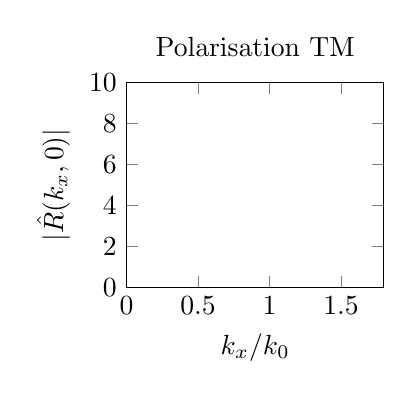
\begin{tikzpicture}[scale=1]
    \begin{axis}[
            title={Polarisation TM},
            ylabel={\(|\hat{R}(k_x,0)|\)},
            xlabel={\(k_x\slash k_0\)},
            width=0.4\textwidth,
            ymin=0,
            ymax=10,
            restrict y to domain=0:+4E+01,
            xmin=0,
            xmax=1.8,
            mark repeat=40,
            legend pos=outer north east
        ]
        % \addplot [color=black,mark=square*] table [col sep=comma, x={s1}, y={Abs(r_ex.11)}] {csv/SOUDAIS/SOUDAIS.r_ex.MODE_2_TYPE_P.csv};
        % % \addlegendentry{Exact};

        % \addplot [color=\ccio,mark=x] table [col sep=comma, x={s1}, y={Abs(r_ibc0.11)}] {csv/SOUDAIS/SOUDAIS.r_ibc.IBC_ibc0_SUC_F_MODE_2_TYPE_P.csv};
        % % \addlegendentry{CI0};

        % \addplot [color=\ccit,mark=diamond*] table [col sep=comma, x={s1}, y={Abs(r_ibc3.11)}] {csv/SOUDAIS/SOUDAIS.r_ibc.IBC_ibc3_SUC_F_MODE_2_TYPE_P.csv};
        % % \addlegendentry{CI3};
    \end{axis}
\end{tikzpicture}
\tikzsetnextfilename{R_SOUDAIS_plan_hoibc.TE}
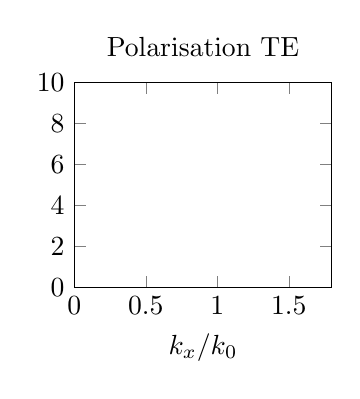
\begin{tikzpicture}[scale=1]
    \begin{axis}[
            title={Polarisation TE},
            ylabel={},
            xlabel={\(k_x\slash k_0\)},
            width=0.4\textwidth,
            xmin=0,
            xmax=1.8,
            ymin=0,
            ymax=10,
            mark repeat=40,
            legend pos=outer north east
        ]
        % \addplot [color=black,mark=square*] table [col sep=comma, x={s1}, y={Abs(r_ex.22)}] {csv/SOUDAIS/SOUDAIS.r_ex.MODE_2_TYPE_P.csv};
        % \addlegendentry{Exact};

        % \addplot [color=\ccio,mark=x] table [col sep=comma, x={s1}, y={Abs(r_ibc0.22)},color=] {csv/SOUDAIS/SOUDAIS.r_ibc.IBC_ibc0_SUC_F_MODE_2_TYPE_P.csv};
        % \addlegendentry{CI0};

        % \addplot [color=\ccit,mark=diamond*] table [col sep=comma, x={s1}, y={Abs(r_ibc3.22)}] {csv/SOUDAIS/SOUDAIS.r_ibc.IBC_ibc3_SUC_F_MODE_2_TYPE_P.csv};
        % \addlegendentry{CI3};
    \end{axis}
\end{tikzpicture}
      %     \caption[CIOE sur empilement de P.~Soudais p.~11]{Module des coefficients diagonaux de \(\mR\) pour \(\eps = 4, \mu = 1, d=0.035\text{m}, f=12\text{GHz}\)}
      %     \label{fig:reflex_fourier:plan:soudais:hoibc}
      % \end{figure}

      La figure \ref{fig:imp_fourier:plan:triple_asymptote:hoibc} montre la limite de la CI3 pour capturer trois asymptotes. Pour cela, il faudrait utiliser une CI d'ordre au moins 6 sur l'opérateur agissant sur \(\vE_t\). La CI3 n'est donc une bonne CIOE que si le nombre d'asymptotes est inférieur à 1, ce que l'on peut calculer connaissant l'empilement (voir proposition \ref{prop:imp_plan:symb_z:1c}).

      Si la matrice d'impédance exacte possède plusieurs asymptotes, il faut autant de pôles à la CIOE pour être une bonne approximation.

      L'expression d'une CIOE vérifiant ce critère est la \hyperlink{ci7}{CI7}
      \begin{equation}
        \left(\oI + \sum_{i=1}^3 \left(d_{i} \left(\frac{\LD}{k_0^2}\right)^i + e_{i} \left(-\frac{\LR}{k_0^2}\right)^i \right)\right)\vE_t = \left(a_0 \oI + \sum_{i=1}^3 \left(b_{i} \left(\frac{\LD}{k_0^2}\right)^i + c_{i} \left(-\frac{\LR}{k_0^2}^i\right) \right)\right)\vJ.
      \end{equation}

      \begin{figure}[!hbt]
          \centering
          \tikzsetnextfilename{Z_triple_asymptote_plan_hoibc.TM}
\begin{tikzpicture}[scale=1]
    \begin{axis}[
            title={Polarisation TM},
            ylabel={\(\Im(\hat{Z}(k_x,0)\)},
            xlabel={\(k_x\slash k_0\)},
            width=0.4\textwidth,
            xmin=0,
            xmax=1.999,
            ymin=-10,
            ymax=10,
            restrict y to domain=-300:300,
            mark repeat=200,
            legend pos=outer north east
        ]
        \addplot [color=black,mark=square*] table [col sep=comma, x={s1}, y={Im(z_ex.tm)}] {csv/triple_asymptote/triple_asymptote.z_ex.MODE_2_TYPE_P.csv};
        % \addlegendentry{Exact};

        \addplot [color=blue,mark=x] table [col sep=comma, x={s1}, y={Im(z_ibc0.tm)}] {csv/triple_asymptote/triple_asymptote.z_ibc.IBC_ibc0_SUC_F_MODE_2_TYPE_P.csv};
        % \addlegendentry{CI0};

        \addplot [color=red,mark=diamond*] table [col sep=comma, x={s1}, y={Im(z_ibc3.tm)}] {csv/triple_asymptote/triple_asymptote.z_ibc.IBC_ibc3_SUC_F_MODE_2_TYPE_P.csv};
        % \addlegendentry{CI3};

        \addplot [color=cyan,mark=pentagon*] table [col sep=comma, x={s1}, y={Im(z_ibc7.tm)}] {csv/triple_asymptote/triple_asymptote.z_ibc.IBC_ibc7_SUC_F_MODE_2_TYPE_P.csv};
        % \addlegendentry{CI7};
    \end{axis}
\end{tikzpicture}
\tikzsetnextfilename{Z_triple_asymptote_plan_hoibc.TE}
\begin{tikzpicture}[scale=1]
    \begin{axis}[
            title={Polarisation TE},
            ylabel={},
            xlabel={\(k_x\slash k_0\)},
            width=0.4\textwidth,
            xmin=0,
            xmax=1.999,
            ymin=-10,
            ymax=10,
            restrict y to domain=-300:300,
            mark repeat=200,
            legend pos=outer north east
        ]
        \addplot [color=black,mark=square*] table [col sep=comma, x={s1}, y={Im(z_ex.te)}] {csv/triple_asymptote/triple_asymptote.z_ex.MODE_2_TYPE_P.csv};
        \addlegendentry{Exact};

        \addplot [color=blue,mark=x] table [col sep=comma, x={s1}, y={Im(z_ibc0.te)}] {csv/triple_asymptote/triple_asymptote.z_ibc.IBC_ibc0_SUC_F_MODE_2_TYPE_P.csv};
        \addlegendentry{CI0};

        \addplot [color=red,mark=diamond*] table [col sep=comma, x={s1}, y={Im(z_ibc3.te)}] {csv/triple_asymptote/triple_asymptote.z_ibc.IBC_ibc3_SUC_F_MODE_2_TYPE_P.csv};
        \addlegendentry{CI3};

        \addplot [color=cyan,mark=pentagon*] table [col sep=comma, x={s1}, y={Im(z_ibc7.te)}] {csv/triple_asymptote/triple_asymptote.z_ibc.IBC_ibc7_SUC_F_MODE_2_TYPE_P.csv};
        \addlegendentry{CI7};                  
    \end{axis}
\end{tikzpicture}
          \caption[CIOE sur empilement avec triple asymptote]{Partie imaginaire des coefficients diagonaux de \(\mZ\) pour \(\eps = 4, \mu = 1, d=0.2\text{m}, f=1\text{GHz}\)}
          \label{fig:imp_fourier:plan:triple_asymptote:hoibc}
      \end{figure}
      \begin{table}[!hbt]
        \centering
        \begin{minipage}[t]{0.49\textwidth}
        \vspace{0pt}
        \centering
        \begin{coefftable}{\hyperlink{ci0}{CI0}}
          \input{csv/triple_asymptote/triple_asymptote.IBC_ibc0_SUC_F_MODE_2_TYPE_P.coeff.txt}
        \end{coefftable}

        \begin{coefftable}{\hyperlink{ci3}{CI3}}
          \input{csv/triple_asymptote/triple_asymptote.IBC_ibc3_SUC_F_MODE_2_TYPE_P.coeff.txt}
        \end{coefftable}
        \end{minipage}
        \tablecoeff[0.49]{\hyperlink{ci7}{CI7}}{csv/triple_asymptote/triple_asymptote.IBC_ibc7_SUC_F_MODE_2_TYPE_P.coeff.txt}
        \caption{Coefficients associés à la figure \ref{fig:imp_fourier:plan:triple_asymptote:hoibc}}
        \label{tab:imp_fourier:plan:triple_asymptote:hoibc}
      \end{table}

\subsection{Problème de la singularité de l'impédance dans le cadre du plan infini pour une couche de matériau sans perte}

Dans la thèse de \cite{aubakirov_electromagnetic_2014}, les constantes de la couche de matériau \(\eps=4,\mu=1,f=12\) GHz, et \(d=3.5\) mm. 
%Ce cas non physique possède un onde guidée pour \((k_x,k_y) = (k_0s^\star,0.)\) où \(\mR(k_0s^\star,0.) = \infty\).

Il existe un \(s_z\) tel que \(\hat\mZ_{ex}(k_0s_z,0.) = \infty\) si \(\eps\mu\in\RR\).
En effet, d'après la formule pour une couche de matériaux de la définition \ref{def:plan:impedance:1c}, 
% \begin{REM}
%   Dis dans le texte (et non seulement dans le titre) que ce n'est possible que si \(\eps\mu\in\RR\).
% \end{REM}
\begin{equation}
  \hat{\mZ}_{ex}(k_x,0.) = i\frac{\eta}{k\sqrt{k^2 - k_x^2}}\tan(\sqrt{k^2 - k_x^2}d)\left(k^2\mI - \hat{\mLR}\right).
\end{equation}
Ainsi, il est facile de voir que l'on a une asymptote à cause de la tangente, et donc pour cet empilement
\begin{equation}
  \label{eq:plan:asymptote_1_couche}
  s_z = \sqrt{\eps \mu - \left(\frac{\pi/2}{k_0 d}\right)^2}.
\end{equation}
% \begin{REM}[asymptote]
%   Et voilà l'explication de \hyperlink{REMnoasymptote}{la precedente remarque}.
% \end{REM}
Le problème est donc que si nous balayons en incidence et que l'on passe par ce point, alors la matrice \(\hat\mZ\) n'est pas définie en ce point.
Or comme le gradient de la fonction est fonction de cette matrice, le gradient n'est pas défini pour tout \(X\).
Si l'on utilise une méthode basée sur le gradient de type Newton, ce que nous avons fait, on comprend pourquoi la méthode numérique échoue à calculer des coefficients.

Dans le code numérique, la discrétisation en incidence et linéaire et nous passions par ce point.
En discrétisant différemment l'incidence, peut-être aurions-nous pu éviter cette difficulté.
\begin{REM}
et une autre méthode de minimisation
\end{REM} 
\begin{REP}
  Question à prévoir.
\end{REP}
\subsubsection{Réduction du nombre de variables de la minimisation}

On décompose alors nos matrices et vecteurs en séparant les parties contentant cette asymptote.

On suppose donc qu'il existe \({\mH}_\infty, {b}_\infty, X_\infty,\) tels que
\begin{align*}
  {\mH} &= {\mH}_\infty + {\mH}_r,
  \\
  {b} &= {b}_\infty + {b}_r,
  \\
  X &= X_\infty + X_r.
\end{align*}

Ces matrices et vecteurs sont reliés par les relations
\begin{align}
  {\mH}_\infty X_\infty &= {b}_\infty,
  \\
  {\mH}_\infty X_r &= 0.
\end{align}

Il faut voir cette décomposition comme deux parties, où l'une est nulle quasiment partout sauf pour le \(s_z\) problématique, et l'autre est définie normalement sauf aux termes correspondant au \(s_z\) où elle est nulle.

Schématiquement, on définit \(i_z\) l'indice d'une ligne telle que \({b}(\hat{\mZ})_{i_z} = \infty\), 

\begin{equation*}
  \begin{matrix}
    {\mH} &=& {\mH}_\infty &+& {\mH}_r,
    \\
    \begin{bmatrix}
      {\mH}_{1,1} & \cdots & {\mH}_{1,N_{CI}}
      \\
      \vdots & \ddots & \vdots
      \\
      {\mH}_{i_z-1,1} & \cdots & {\mH}_{i_z-1,N_{CI}}
      \\
      {\mH}_{i_z,1} & \cdots & {\mH}_{i_z,N_{CI}}
      \\
      {\mH}_{i_z+1,1} & \cdots & {\mH}_{i_z+1,N_{CI}}
      \\
      \vdots & \ddots & \vdots
      \\
      {\mH}_{4N_i,1} & \cdots & {\mH}_{4N_i,N_{CI}}
    \end{bmatrix}
    & = &
    \begin{bmatrix}
      0 & \cdots & 0
      \\
      \vdots & \ddots & \vdots
      \\
      0 & \cdots & 0
      \\
      {\mH}_{i_z,1} & \cdots & {\mH}_{i_z,N_{CI}}
      \\
      0 & \cdots & 0
      \\
      \vdots & \ddots & \vdots
      \\
      0 & \cdots & 0
    \end{bmatrix}
    & + & 
    \begin{bmatrix}
      {\mH}_{1,1} & \cdots & {\mH}_{1,N_{CI}}
      \\
      \vdots & \ddots & \vdots
      \\
      {\mH}_{i_z-1,1} & \cdots & {\mH}_{i_z-1,N_{CI}}
      \\
      0 & \cdots & 0
      \\
      {\mH}_{i_z+1,1} & \cdots & {\mH}_{i_z+1,N_{CI}}
      \\
      \vdots & \ddots & \vdots
      \\
      {\mH}_{4N_i,1} & \cdots & {\mH}_{4N_i,N_{CI}}
    \end{bmatrix}
  \end{matrix}.
\end{equation*}
Dans les faits, \({\mH}_\infty\) a \(4\) lignes non nulles et \({\mH}_r\) en a autant de nulles aux mêmes endroits.


On développe donc la fonction
% \begin{REM}
%   Voir \hyperlink{REMfonction}{avant}.
%   De plus, il est préférable de l'écrire sur le carré de la norme.
% \end{REM}
% \begin{REP}
%   Fait
% \end{REP}
suivant cette décomposition :
\begin{align*}
\argmin{X}\left\rVert {\mH} X - {b} \right \rVert^2 &= \argmin{X_r}\left\rVert \left({\mH}_\infty + {\mH}_r\right)\left( X_\infty + X_r \right) - {b}_\infty - {b}_r \right \rVert^2.
\\
\intertext{On utilise la relation entre \({\mH}_\infty X_\infty\) et \({b}_\infty\)}
&=  \argmin {X_r}\left\rVert {\mH}_\infty X_r + {\mH}_r X_\infty + {\mH}_r X_r - {b}_r \right \rVert^2.
\\
\intertext{Enfin par définition de \({\mH}_\infty\) et \(X_r\), leur produit est nul}
&= \argmin{X_r} \left\rVert {\mH}_r ( X_r + X_\infty)- {b}_r \right \rVert^2.
\end{align*}

On voit alors que l'on peut résoudre le problème
% \begin{REM}
%   Ce n'est pas rigoureux
% \end{REM}
% \begin{REP}
%   Pourtant c'est issus du travail à Montréal.
% \end{REP}
si l'on minimise uniquement sur les \(X_r\), les autres étant fixés, et si l'on enlève du système les lignes où l'impédance n'est pas définie.

\subsubsection{Application de la réduction à la CI3}

On rappelle l'expression de la CI3
\begin{equation*}
  \hat{\mZ}_{ap}(k_x,0) = \left(\mI + b_1 \hat{\mLD}(k_x,0) - b_2 \hat{\mLR}(k_x,0) \right)^{-1}\left(a_0\mI + a_1 \hat{\mLD}(k_x,0) - a_2 \hat{\mLR}(k_x,0) \right).
\end{equation*}

% On voit donc que pour faire apparaître une asymptote,
% \begin{REM}
%   Pas math. "Une condition nécessaire et suffisante pour que \(\mZ\) ai une asymptote est".
%   Elle est peut être seulement nécessaire car si \(a_0\mI + a_1\mLD -a_2\mLR\) a un noyau
% \end{REM}
% \begin{REP}
%   FAIT
% \end{REP}
Une condition nécessaire et suffisante pour que \(\hat{\mZ}_{ap}\) ait une asymptote est que la matrice de gauche ne soit pas inversible en \(s_z\).

La matrice \({\mH}_\infty\) est donc nulle partout sauf en 8 termes, placés sur les deux dernières colonnes et les 4 lignes correspondantes à \((k_x,k_y)=(k_0 s_z,0)\).

Connaissant les expressions des matrices \(\hat\mLD,\hat\mLR\) introduites dans la partie précédente alors on déduit que
\begin{align*}
  X_\infty = \begin{bmatrix}
    0\\
    0\\
    0\\
    (k_0 s_z)^{-2}\\
    (k_0 s_z)^{-2}\\
  \end{bmatrix},
  & &
  X_r = \begin{bmatrix}
  a_0\\
  a_1\\
  a_2\\
  0\\
  0\\
  \end{bmatrix}.
\end{align*}

\subsection{Choix de la méthode numérique pour résoudre la minimisation sous contraintes}

  Des méthodes basées sur le gradient sont adaptées, car la fonction est dérivable pour tout \(X\) et les contraintes se comportent comme des polynômes dépendant uniquement des composantes de \(X\). Nous avons donc fait le choix de la méthode \gls{acr-sqp} pour les raisons suivantes:
 
  \begin{itemize}
    \item elle est éprouvée depuis \cite{kraft_software_1988} et des sources Fortran à jour sont disponibles à \url{https://github.com/jacobwilliams/slsqp}, ce qui est capital pour l'intégrer dans un code industriel ;
    \item elle est rapide, nous avons observé que cette méthode convergeait en quelques dizaines d'itérations au plus ;
    \item elle accepte des contraintes non linéaires, donc elle est adaptée à nos CSU.
  \end{itemize}

% \subsection{Résultats numérique avec contraintes}

  % \begin{REM}
  %   Quelques résultats avec contraintes
  % \end{REM}

\section{Calcul des coefficients de la CI3 par moindres carrés sur les coefficients de la série de Fourier}

  On peut aussi résoudre calculer les coefficients en minimisant l'erreur entre les coefficients de Fourier.

  Soit \(\mM_A\) et \(\mM_B\) les fonctions introduites à la définition \ref{def:plan:matrices_MA-MB} et \(\hat\mR\) la fonction définie en \ref{def:plan:reflexion:impedance}.

  \begin{defn}%[]
    \label{def:plan:minimisation:matrices_MR}
    On définit les fonctions \(\hat\mR_{ex}, \hat\mR_{CI3}\) de \(\RR\times\RR\times \rightarrow \mathcal{M}_2(\CC)\) telles que
    \begin{align*}
      \hat\mR_{ex}(k_x,k_y) &= \hat\mR(k_x,k_y, \hat\mZ_{ex}(k_x,k_y))
      \\
      \hat\mR_{CI3}(k_x,k_y) &= \hat\mR(k_x,k_y, \hat\mZ_{CI3}(k_x,k_y))
    \end{align*}
    où \(\hat\mZ_{ex},\hat\mZ_{CI3}\) sont des fonctions définies à la proposition \ref{prop:plan:synthese:impedance} et à l'équation \eqref{eq:plan:hoibc:ci3}.
  \end{defn}

  \subsection[Expression de la fonctionnelle JR]{Expression de la fonctionnelle \(J_R\)}

    On utilise les fonctions \(\mN_E, \mN_H\) introduites à la définition \ref{def:plan:matrices_NE-NH} et \(\hat\mLD,\hat\mLR\) définies aux définitions \ref{eq:plan:fourier:LD}-\ref{eq:plan:fourier:LR}.

    \begin{defn}
      On définit \(\mA_0,\mA_1,\mA_2,\mA_2,\mB_1,\mB_2\) les fonctions de \(\RR \times \RR \times \mathcal{M}_2(\CC) \rightarrow \ \mathcal{M}_2(\CC)\) telles que        
      \begin{align*}
        \mA_0(k_x,k_y,\mR) &= \mN_E(k_x,k_y,0^+,\mR)
        \\
        \mA_1(k_x,k_y,\mR) &= \hat{\mLD}(k_x,k_y)\mN_E(k_x,k_y,0^+,\mR)
        \\
        \mA_2(k_x,k_y,\mR) &= -\hat{\mLR}(k_x,k_y)\mN_E(k_x,k_y,0^+,\mR)
        \\
        \mB_1(k_x,k_y,\mR) &= \hat{\mLD}(k_x,k_y)\mN_H(k_x,k_y,0^+,\mR)
        \\
        \mB_2(k_x,k_y,\mR) &= -\hat{\mLR}(k_x,k_y)\mN_H(k_x,k_y,0^+,\mR)            
      \end{align*}

      On définit \(\tilde{\mH}_{CI3}\) la fonction de \(\RR \times \RR \times \mathcal{M}_2(\CC) \rightarrow \mathcal{M}_{4\times5}(\CC)\) telle que
      \begin{align*}
        & \tilde\mH_{CI3}(k_x,k_y,\mR) =  \\ &
        \begin{bmatrix}
          \mA_0(k_x,k_y,\mR)_{11} & \mA_1(k_x,k_y,\mR)_{11} & \mA_2(k_x,k_y,\mR)_{11} & \mB_1(k_x,k_y,\mR)_{11} & \mB_2(k_x,k_y,\mR)_{11}
          \\
          \mA_0(k_x,k_y,\mR)_{12} & \mA_1(k_x,k_y,\mR)_{12} & \mA_2(k_x,k_y,\mR)_{12} & \mB_1(k_x,k_y,\mR)_{12} & \mB_2(k_x,k_y,\mR)_{12}
          \\
          \mA_0(k_x,k_y,\mR)_{21} & \mA_1(k_x,k_y,\mR)_{21} & \mA_2(k_x,k_y,\mR)_{21} & \mB_1(k_x,k_y,\mR)_{21} & \mB_2(k_x,k_y,\mR)_{21}
          \\
          \mA_0(k_x,k_y,\mR)_{22} & \mA_1(k_x,k_y,\mR)_{22} & \mA_2(k_x,k_y,\mR)_{22} & \mB_1(k_x,k_y,\mR)_{22} & \mB_2(k_x,k_y,\mR)_{22}
        \end{bmatrix}
      \end{align*}

      On définit \(\tilde{b}\) la fonction de \(\RR \times \RR \times \mathcal{M}_2(\CC) \rightarrow \mathcal{M}_{4\times1}(\CC)\) telle que
      \begin{equation*}
        \tilde{b}(k_x,k_y,\mR) = -
        \begin{bmatrix}
          \mN_H(k_x,k_y,0^+,\mR)_{11}
          \\
          \mN_H(k_x,k_y,0^+,\mR)_{12}
          \\
          \mN_H(k_x,k_y,0^+,\mR)_{21}
          \\
          \mN_H(k_x,k_y,0^+,\mR)_{22}
        \end{bmatrix}
      \end{equation*}
    \end{defn}

    \begin{prop}
      Soit \(X = (a_0,a_1,a_2,b_1,b_2)\), \((k_x,k_y)\) fixé et \(\hat\mR_{ex}\) la matrice définie en \ref{def:plan:minimisation:matrices_MR}, alors
      \begin{multline*}
        \argmin{X\in\CC^5} \norm{\hat\mR_{CI3}(k_x,k_y,X) - \hat\mR_{ex}(k_x,k_y)} =
        \\
        \argmin{X\in\CC^5} \norm{\tilde{\mH}_{CI3}(k_x,k_y,\hat\mR_{ex}(k_x,k_y))X - \tilde{b}(k_x,k_y,\hat\mR_{ex}(k_x,k_y))}
      \end{multline*}
    \end{prop}

    \begin{proof}
      C'est la même méthodologie que pour l'impédance.
      On rappelle de la section précédente
      \begin{multline*}
        \hat{\mZ}_{CI3}(k_x,k_y) = \left(\mI + b_1 \hat{\mLD}(k_x,k_y) - b_2 \hat{\mLR}(k_x,k_y) \right)^{-1}
        \\
        \left(a_0 \mI + a_1 {\hat{\mLD}(k_x,k_y)} - a_2 {\hat{\mLR}(k_x,k_y)}\right)
      \end{multline*}
      On pose \(\hat\mZ_D(k_x,k_y) = \mI + b_1 \hat{\mLD}(k_x,k_y) - b_2 \hat{\mLR}(k_x,k_y)\) et \(\hat\mZ_N(k_x,k_y) = a_0 \mI + a_1 {\hat{\mLD}(k_x,k_y)} - a_2 {\hat{\mLR}(k_x,k_y)}\) donc

      \begin{align*}
        &{\hspace{1em}}~ \argmin{X\in\CC^5} \norm{\hat\mR_{CI3}(k_x,k_y,X) - \hat\mR_{ex}(k_x,k_y)}
        \\
        & = \argmin{X\in\CC^5} \norm{ - \mM_B(k_x,k_y,0^+,\hat\mZ_{CI3})^{-1}\mM_A(k_x,k_y,0^+,\hat\mZ_{CI3})- \hat\mR_{ex}(k_x,k_y) }
        \\
        & = \argmin{X\in\CC^5} \norm{ - \mM_B(k_x,k_y,0^+,\hat\mZ_{CI3})^{-1}\left(\mM_A(k_x,k_y,0^+,\hat\mZ_{CI3}) +  \mM_B(k_x,k_y,0^+,\hat\mZ_{CI3})\hat\mR_{ex}(k_x,k_y)\right) }      
        \\ 
        & = \argmin{X\in\CC^5} \norm{\mM_A(k_x,k_y,0^+,\hat\mZ_{CI3}) +\mM_B(k_x,k_y,0^+,\hat\mZ_{CI3})\hat\mR_{ex}(k_x,k_y)}
        \intertext{D'après la définition \ref{def:plan:matrices_MA-MB} des fonctions \(\mM_A, \mM_B\),}
        & = \argmin{X\in\CC^5} \left\lVert \left(\mJ_E(k_x,k_y,0^+)-\hat\mZ_{CI3}(k_x,k_y)\mJ_H(k_x,k_y,0^+)\right) \right.
        \\
        & \qquad \qquad \quad + \left.\left(\mH_E(k_x,k_y,0^+)-\hat\mZ_{CI3}(k_x,k_y)\mH_H(k_x,k_y,0^+)\right)\hat\mR_{ex}(k_x,k_y) \right\lVert
        \intertext{D'après la définition de \(\hat\mZ_{CI3}\),}        
        & = \argmin{X\in\CC^5} \left\lVert \hat\mZ_D(k_x,k_y)^{-1}\left(\hat\mZ_D(k_x,k_y)\mJ_E(k_x,k_y,0^+)-\hat\mZ_N(k_x,k_y)\mJ_H(k_x,k_y,0^+)\right) \right.
        \\
        & \qquad \qquad \quad + \left.\hat\mZ_D(k_x,k_y)^{-1}\left(\hat\mZ_D(k_x,k_y)\mH_E(k_x,k_y,0^+)-\hat\mZ_N(k_x,k_y)\mH_H(k_x,k_y,0^+)\right)\hat\mR_{ex}(k_x,k_y) \right\lVert
        \\
        & = \argmin{X\in\CC^5} \left\lVert \left(\hat\mZ_D(k_x,k_y)\mJ_E(k_x,k_y,0^+)-\hat\mZ_N(k_x,k_y)\mJ_H(k_x,k_y,0^+)\right) \right.
        \\
        & \qquad \qquad \quad + \left.\left(\hat\mZ_D(k_x,k_y)\mH_E(k_x,k_y,0^+)-\hat\mZ_N(k_x,k_y)\mH_H(k_x,k_y,0^+)\right)\hat\mR_{ex}(k_x,k_y) \right\lVert
        \intertext{D'après la définition \ref{def:plan:matrices_NE-NH} des fonctions \(\mN_E, \mN_H\),}        
        & = \argmin{X\in\CC^5} \norm{\hat\mZ_N(k_x,k_y)\mN_E(k_x,k_y,0^+,\hat\mR_{ex}(k_x,k_y)) + \hat\mZ_D(k_x,k_y)\mN_H(k_x,k_y,0^+,\hat\mR_{ex}(k_x,k_y))}
      \end{align*}
      et l’on conclut d'après la définition des fonctions \(\hat\mZ_D, \hat\mZ_N\).
    \end{proof}

    \begin{defn}
      On définit \(\tilde{\mA}_{CI3}\) la matrice de \(\mathcal{M}_{4N_{n}N_{k_z}\times5}(\CC)\) telle que
      \begin{equation*}
        \tilde{\mA}_{CI3} = 
        \begin{bmatrix}
          \tilde\mH_{CI3}(n_1,k_{z1},\hat\mR_{ex}(n_1,k_{z1}))
          \\
          \vdots
          \\
          \tilde\mH_{CI3}(n_i,k_{zj},\hat\mR_{ex}(n_i,k_{zj}))
          \\
          \vdots
          \\
          \tilde\mH_{CI3}(n_{N_n},k_{zN_{k_z}},\hat\mR_{ex}(n_{N_n},k_{zN_{k_z}}))
        \end{bmatrix}
      \end{equation*}
      On définit \(\tilde{g}\) le vecteur colonne \(\CC^{4N_{n}N_{k_z}}\) telle que
      \begin{equation*}
        \tilde{g} = 
        \begin{bmatrix}
          \tilde{b}(n_1,k_{z1},\hat\mR_{ex}(n_1,k_{z1}))
          \\
          \vdots
          \\
          \tilde{b}(n_i,k_{zj},\hat\mR_{ex}(n_i,k_{zj}))
          \\
          \vdots
          \\
          \tilde{b}(n_{N_n},k_{zN_{k_z}},\hat\mR_{ex}(n_{N_n},k_{zN_{k_z}}))
        \end{bmatrix}
      \end{equation*}
    \end{defn}

    On peut alors calculer les coefficients de la CI3

    \begin{defn}
      On définit la fonctionnelle \(J_R\)
      \begin{equation*}
        J_R(X) = \norm{\tilde{\mA}_{CI3}X - \tilde{g}}
      \end{equation*}
    \end{defn}

    \begin{thm}[Minimisation sans contraintes pour la CI3]

      Les coefficients de la CIOE sont solutions du problème

      Trouver \(X^* \in \CC^5\) tel que
      \begin{equation*}
        X^* = \argmin{X\in \CC^5} J_R(X)
      \end{equation*}
    \end{thm}

    \begin{prop}
      Si \(\conj{\tilde{\mA}_{CI3}^t}\tilde{\mA}_{CI3}\) est inversible alors
      \begin{equation*}
        X^* = (\conj{\tilde{\mA}_{CI3}^t}\tilde{\mA}_{CI3})^{-1}\conj{\tilde{\mA}_{CI3}^t}\tilde{g}
      \end{equation*}
    \end{prop}
    \begin{proof}
      Même méthode que pour la proposition \ref{prop:plan:minimisation:minimum_sans_contraintes} sur l'impédance.
    \end{proof}

    Nous n'avons pas réussi à démontrer que cette matrice était définie pour tout empilement et toute incidence, pas même pour des CIOE plus simples.

    \begin{thm}[Minimisation avec contraintes pour la CI3]

      Soit \(\CSU[3]{CI3}\) le sous-espace de \(\CC^5\) issu de la définition \ref{def:csu:ci3-3}.
      Alors les coefficients de la CIOE respectant les CSU sont solutions du problème

      Trouver \(X^* \in \CC^5\) tel que
      \begin{equation*}
        X^* = \argmin{X\in \CSU[3]{CI3}} J_R(X)
      \end{equation*}
    \end{thm}

    


\sectionstar{Conclusion}
Nous avons proposé une méthode pour calculer des coefficients complexes vérifiant une des CSU choisie, et qui permettent d'approcher l'opérateur de Calderón dans le cas d'un objet plan infini en minimisant au sens des moindres carrés la différence entre les matrices d'impédance exactes et approchées.

Nous avons montré que minimiser l'erreur entre les matrices de réflexion aboutit aux mêmes coefficients de CIOE.
\begin{REM}
	donc on a, à un ordre donné, unicité de la CIOE?
\end{REM} 
Pour cela, nous avons réalisé une analyse spectrale des équations de Maxwell et montré que la condition d'impédance s'exprime comme un multiplicateur de Fourier matriciel, tout comme la matrice de réflexion.
Grâce à cette analyse spectrale, nous avons aussi exprimé les CIOE comme des multiplicateurs de Fourier matriciels dont on a déduit la matrice de réflexion associée.
Nous avons alors exprimé le problème de minimisation sous contraintes et montré que celui-ci a besoin d'être réduit dans le cas d'une couche de matériau sans pertes.
\begin{REM}
  en fait, elle est là l’originalité du travail.
  On ne fait les sempiternelles approximations (Taylor ou Padé), on minimise. C'est ça ?
\end{REM} 
Nous avons montré sur cette géométrie que la CIOE choisie, la \hyperlink{ci3}{CI3}, était largement plus précise que les précédentes \hyperlink{ci01}{CI01} et \hyperlink{ci1}{CI1}.
Ce gain en précision est tel que l'on peut introduire des contraintes lors du calcul et avoir une solution finale convenable, relativement à l'opérateur exact.
